%%%%%%%%%%%%%%%%%%%%%%%%%%%%%%%%%%%%%%%%%%%%%%%%%%%%%%%%%%%%%%%%%%%%
%% I, the copyright holder of this work, release this work into the
%% public domain. This applies worldwide. In some countries this may
%% not be legally possible; if so: I grant anyone the right to use
%% this work for any purpose, without any conditions, unless such
%% conditions are required by law.
%%%%%%%%%%%%%%%%%%%%%%%%%%%%%%%%%%%%%%%%%%%%%%%%%%%%%%%%%%%%%%%%%%%%

\documentclass[
  printed, %% The `digital` option enables the default options for the
           %% digital version of a document. Replace with `printed`
           %% to enable the default options for the printed version
           %% of a document.
  color,   %% Uncomment these lines (by removing the %% at the
%%           %% beginning) to use color in the digital version of your
%%           %% document
  table,   %% The `table` option causes the coloring of tables.
           %% Replace with `notable` to restore plain LaTeX tables.
  oneside, %% The `twoside` option enables double-sided typesetting.
           %% Use at least 120 g/m² paper to prevent show-through.
           %% Replace with `oneside` to use one-sided typesetting;
           %% use only if you don’t have access to a double-sided
           %% printer, or if one-sided typesetting is a formal
           %% requirement at your faculty.
  lof,     %% The `lof` option prints the List of Figures. Replace
           %% with `nolof` to hide the List of Figures.
  lot,     %% The `lot` option prints the List of Tables. Replace
           %% with `nolot` to hide the List of Tables.
  %% More options are listed in the user guide at
  %% <http://mirrors.ctan.org/macros/latex/contrib/fithesis/guide/mu/fi.pdf>.
]{fithesis3}
%% The following section sets up the locales used in the thesis.
\usepackage[resetfonts]{cmap} %% We need to load the T2A font encoding
\usepackage[T1,T2A]{fontenc}  %% to use the Cyrillic fonts with Russian texts.
\usepackage[
  main=english, %% By using `czech` or `slovak` as the main locale
                %% instead of `english`, you can typeset the thesis
                %% in either Czech or Slovak, respectively.
  english, german, russian, czech, slovak %% The additional keys allow
]{babel}        %% foreign texts to be typeset as follows:
%%
%%   \begin{otherlanguage}{german}  ... \end{otherlanguage}
%%   \begin{otherlanguage}{russian} ... \end{otherlanguage}
%%   \begin{otherlanguage}{czech}   ... \end{otherlanguage}
%%   \begin{otherlanguage}{slovak}  ... \end{otherlanguage}
%%
%% For non-Latin scripts, it may be necessary to load additional
%% fonts:
\usepackage{paratype}
\def\textrussian#1{{\usefont{T2A}{PTSerif-TLF}{m}{rm}#1}}
%%
%% The following section sets up the metadata of the thesis.
\thesissetup{
    date        = \the\year/\the\month/\the\day,
    university  = mu,
    faculty     = fi,
    type        = bc,
    author      = Petr Zelina,
    gender      = m,
    advisor     = {doc. RNDr. Aleš Horák, Ph.D.},
    title       = {Pretraining and Evaluation of Czech ALBERT Language Model},
    TeXtitle    = {Pretraining and Evaluation of Czech ALBERT Language Model},
    keywords    = {NLP, Czech NLP, neural networks, deep neural networks, deep learning, transformers, BERT, ALBERT, text classification, question answering},
    TeXkeywords = {NLP, Czech NLP, neural networks, deep neural networks, deep learning, transformers, BERT, ALBERT, text classification, question answering},
    abstract    = {%
        This thesis explores a new language model called ALBERT, released by Google Research in 2019. The ALBERT architecture has been very successful in English NLP tasks and this thesis tests its utilization for the Czech language.
        
        % The work gives an overview of the models leading to ALBERT and their design. Further, it shares the process of creation of several Czech ALBERT models. Finally, it evaluates their performance and compares them to the current Czech state-of-the-art models on text classification and question answering tasks.

        We give an overview of the models leading to ALBERT and their design. Further, we share the creation process of several Czech ALBERT models. Finally, we evaluate their performance and compare them to the current Czech state-of-the-art models on text classification and question answering tasks. 

        % ALBERT models have been very successful in English NLP tasks and this thesis tests the feasibility of the ALBERT architecture for the Czech language. We give an overview of the models leading to ALBERT and their design. Further, we share the process of creation of several Czech ALBERT models. Finally, we evaluate the their performance and compare them to the current Czech state-of-the-art models on text classification and question answering tasks. 
        
       
    },
    thanks      = {%
        I would like to thank my supervisor, doc. RNDr. Aleš Horák, Ph.D., for his guidance through the process and helpful remarks, and Ronald Luc for fruitful discussions.
        
        I am also very grateful to my family who supported me the whole time.
    
        \vspace{1em}
        {\parindent=0cm
        Computational resources for this work were supplied by the project "e-Infrastruktura CZ" (e-INFRA LM2018140) provided within the program Projects of Large Research, Development and Innovations Infrastructures.
        }
    },
    bib         = {bib.bib},
    %% Uncomment the following line (by removing the %% at the
    %% beginning) and replace `assignment.pdf` with the filename
    %% of your scanned thesis assignment.
    assignment         = {},
}

% Tato práce se zabývá novým jazykovým modelem nazvaným ALBERT, který byl vydaný společností Google Research v roce 2019. Architektura ALBERT je velmi úspěšná ve zpracování anglických jazykových problémů a tato práce testuje možnosti jejího využití pro český jazyk.

% Nejdříve rozebíráme vývoj a strukturu modelu ALBERT. Dále se zabýváme návrhem a trénováním českých modelů. Nakonec porovnáváme jejich úspěšnost s aktuálními českými řešeními na úlohách jako je klasifikace textu nebo automatické odpovídání na otázky.

% Práce nejdříve rozebírá vývoj a strukturu modelu ALBERT. Dále se zabývá návrhem a trénováním několika českých modelů. Nakonec porovnává jejich úspěšnost s aktuálními českými řešeními na úlohách, jako je klasifikace textu nebo automatické hledání odpovědí.

% , a možnostmi jeho využití pro češtinu.


\usepackage[utf8]{inputenc}
\usepackage[hypcap=true,font={small}]{caption}
\usepackage{adjustbox}
\usepackage{multirow}
\usepackage{makecell}
\usepackage{dirtytalk}

\usepackage{makeidx}      %% The `makeidx` package contains
\makeindex                %% helper commands for index typesetting.
%% These additional packages are used within the document:
\usepackage{paralist} %% Compact list environments
\usepackage{amsmath}  %% Mathematics
\usepackage{amsthm}
\usepackage{amsfonts}
\usepackage{url}      %% Hyperlinks
\usepackage{markdown} %% Lightweight markup
\usepackage{tabularx} %% Tables
\usepackage{tabu}
\usepackage{booktabs}
\usepackage{listings} %% Source code highlighting
\lstset{
  basicstyle      = \ttfamily,
  identifierstyle = \color{black},
  keywordstyle    = \color{blue},
  keywordstyle    = {[2]\color{cyan}},
  keywordstyle    = {[3]\color{olive}},
  stringstyle     = \color{teal},
  commentstyle    = \itshape\color{magenta},
  breaklines      = true,
}
\usepackage{floatrow} %% Putting captions above tables
\floatsetup[table]{capposition=top}
%% The following code fixes the rendering of BibLaTeX ISO 690
%% references in old TeX Live (such as the one at Overleaf).
\thesisload
\makeatletter
\def\thesis@biblatexiso@fix@package{iso-numeric.bbx}
\def\thesis@biblatexiso@fix@end{\relax}
\newif\ifthesis@biblatexiso@fix@
\thesis@biblatexiso@fix@false
\def\thesis@biblatexiso@fix@next#1,{%
  \def\thesis@biblatexiso@fix@current{#1}%
  \ifx\thesis@biblatexiso@fix@current\thesis@biblatexiso@fix@package
    \thesis@biblatexiso@fix@true
  \fi
  \ifx\thesis@biblatexiso@fix@current\thesis@biblatexiso@fix@end
    \expandafter
    \@gobble
  \fi
  \thesis@biblatexiso@fix@next
}
\expandafter\expandafter\expandafter\thesis@biblatexiso@fix@next\@filelist,\relax,
\ifthesis@biblatexiso@fix@
  \defbibenvironment{bibliography}
    {\list%
       {\MethodFormat}%
       {\setlength{\labelwidth}{\labelnumberwidth}%
        \setlength{\leftmargin}{\labelwidth}%
        \setlength{\labelsep}{\biblabelsep}%
        \addtolength{\leftmargin}{\labelsep}%
        \setlength{\itemsep}{\bibitemsep}%
        \setlength{\parsep}{\bibparsep}}%
        \renewcommand*{\makelabel}[1]{\hss##1}
        }%
    {\endlist}%
  {\item}%
\fi


\hyphenation{ALBERT}


\makeatother
\begin{document}
\chapter*{Introduction}
% \chapter*{Pretraining and Evaluation of Czech ALBERT Language Model}
\addcontentsline{toc}{chapter}{Introduction}


%context
In 2018, researchers from Google released a new language model called BERT~\parencite{bert}. It quickly rose to the top of the leaderboards of many English NLP tasks such as question answering or sentiment analysis. Later, in 2019, they released a leaner version called ALBERT~\parencite{albert}, which is faster and much smaller, and achieves even better performance.

%goals
This thesis aims to pretrain an ALBERT model for the Czech language, evaluate its efficiency in several extrinsic tasks, and compare the results to other current state-of-the-art Czech NLP models. 

There are two BERT models with multilingual support that include the Czech language. These are included in the evaluation as well.

The first evaluated downstream task is the classification of various attitudes and manipulative techniques in text from the Czech Propaganda dataset~\parencite{propaganda}. 

The second task is question answering from the Czech Simple Question Answering Database (SQAD)\parencite{sqad}. Given a paragraph and a question, the goal is to select the best answer to the question from the context paragraph.

%structure
The first chapter focuses on the most common approaches for applying deep artificial neural networks to NLP tasks. The second chapter describes the evolution and architecture of language models leading to ALBERT. The third chapter analyzes the development of the Czech ALBERT model. The evaluation process and results are described in the fourth chapter.

%tools
The implementation of the Czech ALBERT is based on this GitHub repository~\parencite{albert_repo}, written in TensorFlow v1.15 and Python 3.6. The source code can be found here \parencite{thesis_repo}. Trained ALBERT models can be downloaded from \url{https://nlp.fi.muni.cz/projekty/czech_albert/}.

% %results
% I was able to create a pipeline and to pretrain several Czech ALBERT models. Due to the significant processing resource  requirements of this architecture, I was not able to achieve similar base performance as that of the original English models, even though I utilized the Czech cloud computing infrastructure MetaCentrum \parencite{metacentrum}. Nevertheless, the performance on several downstream Czech NLP tasks was comparable to the performance of the state-of-the-art models. I am confident that with more powerful hardware and longer pretraining time, these models could perform even better.

The resulting models are easily adaptable for a broad range of tasks using, for example, the Keras framework.

% ####################################
% ####################################

\chapter{Deep learning and NLP}
For a long time, natural language processing was dominated by systems with human-created rules. These systems are often complex, incomplete, their creation is labor-intensive, and they are hard to expand. Machine learning offers solutions to some of these problems, but it comes with its own challenges.

Even though machine learning approaches to NLP tasks existed, they were often based on shallow models (such as logistic regression or SVM) \parencite{deepNLP}. Part of the reason was the lack of processing power. The other problem is that machine learning expects numbers, but NLP tasks are word-based problems. The most common approach was to encode the words as one-hot vectors, meaning the word is encoded to a vector with the size of the whole dictionary, and all but one component are 0.  These high dimensional sparse vectors cause many problems, and the situation is even worse for morphologically rich languages.

We know that deep learning\parencite{deepNLP} is successful in many areas, like image recognition or various prediction and classification tasks. From this, we can assume that it can be effective in NLP.

In the last few years with the increases in processing power, there have been several breakthroughs that made deep learning for NLP feasible, and even successful.

\section{Sequence processing}
Language is intrinsically sequential. A traditional way of processing sequences in deep learning is with the use of recurrent neural networks (RNNs). They process the inputs one by one and propagate an internal state across the whole sequence. They are thus able to deal with sequences of variable length. 

A big problem with simple RNNs was the vanishing gradient problem. Because of the architecture of the network and the nature of backpropagation, their memory is limited. LSTM (Long short-term memory) \parencite{lstm}, \parencite{lstm-info} is a type of an RNN that avoids this problem by using a kind of memory cells, which can be implemented as a neural network component and are trainable.

Another issue is the necessity to process the input sequentially. This reduces their parallelizability. 

\section{Word embeddings}
Today most models tackle the high dimensionality problem by using word embeddings \parencite{mikolov}. Word embeddings are a simple way of decreasing the dictionary dimension. Each word has its own embedding, which is a real vector of relatively low dimension (e.g. 300 instead of 100\,000 for one-hot encoding). The embeddings of all words in the dictionary form a vector space, where words with similar meaning are close together. Even better, if some assumptions are satisfied \parencite{vectadd}, the vectors can be added and subtracted from each other in a meaningful way.  

Word embeddings are usually trained unsupervised in advance on a big corpus. The training objective is to predict which words occur in a similar context. The most common methods for training word embeddings are skip-gram and continuous bag-of-words described by Mikolov et al.~\parencite{mikolov}. The resulting weights than can be used as an initialization for the first layer of the final model.

The main drawback is that these embeddings cannot distinguish polysemy, where the same word can have multiple different meanings. For example, the word mouse as an animal and as a pointing device used with a computer. If one meaning is more common than the other, the model usually ignores the other meaning. However, when the occurrence is similar, then the vector representation can end up somewhere in between both meanings, which is not useful.

\section{Contextualized word embeddings}
To solve the problem with simple word embeddings and polysemy, we need to create a more complex model. A single word by itself is not enough to infer its exact meaning. We need to consider its context while encoding it. 

In many languages, the context of a given word may be many words apart. It is not sufficient to consider only a small window around the word. Including the context requires more complex architectures with more parameters. These big networks than can have the ability to comprehend the language more than just expressing the meaning of a single word. We can use their representations to infer things about whole sentences or paragraphs. Because they are no longer simple embeddings, we call them language models.


% ####################################
% ####################################

\chapter{Language models}
This chapter shows some of the approaches and architectures for creating more complex language models.

\section{Language models and transfer learning}
For many NLP tasks, it is crucial to understand the underlying system of the language. This system is often complicated. Generally, it is hard to gather a large amount of data for the specific task we want the model to learn. Because of this, models trained from scratch only on the task data are usually not able to comprehend the language and are less accurate.

That is where the idea of transfer learning comes from. We can first pretrain a general language model on big and relatively easy-to-create corpora so that it can learn the inner language structure. Then we can fine-tune the model for the specific task. It has been shown that this approach can increase the quality of the resulting model \parencite{transfer1}, \parencite{transfer2}.

Traditionally, language models in NLP were viewed simply from a statistical point of view as a probability distribution over sequences of words/tokens. Well-formed sentences had a higher probability than nonsensical ones. They could be used, for example, for rating possible answers or text generation. The models described below are more powerful. They contain a deeper understanding of the language, and we can use their inner language representation as a start-point for almost any NLP task.

 \section{ELMo}
One of the first deep bidirectional word embeddings is ELMo~(Embeddings from Language Models)~\parencite{elmo}. ELMo applies a BiLSTM approach, that means it uses two deep recurrent LSTM networks, one which scans from front to back, and the other which scans from back to front. The resulting embedding is a linear combination of the hidden states of both LSTMs at the time each one scanned the word in question (Figure \ref{fig:contextual_models}). The problem this model has is that it is not designed to use deep architecture to consider the context on both sides at once because both LSTMs see only in one direction and are trained independently. 

\section{Transformers and attention}
\label{sec:transformer}
Transformer is a neural network architecture whose goal is to transform one sequence to another. It is very effective, for example, in machine translation. Transformers were presented by Vaswani et al. in 2018 \cite{attentionisall}.

Unlike RNNs, transformers can see the whole input sequence at the same time. However, this means they have to process a lot of information all at once. When humans try to make sense of a complex sentence, they do not read it all at once, but they usually focus on different parts based on the current word/phrase they are reading. Attention is a mechanism, which allows transformers to do something similar.

\subsection{Architecture}

The input of the transformer is a sequence of one-hot encoded words. The first layer of the transformer is a word embedding to a lower dimension, which is initialized randomly. There is no need to pretrain this embedding, it gets trained with the whole model. 
The embedded words are then fed into a sequence of encoder layers, which creates a hidden representation of the input sequence at its end. The hidden state is then used in a series of decoder layers, which create the final output sequence.

A great in-depth explanation can be found in a blog post by Jay Alammar called The Illustrated Transformer  \parencite{ilustrtran}.

\subsection{Encoder layer}
\label{sec:encoder}
Encoder layer consists of two sublayers: multi-head self-attention layer and feed-forward layer.

\subsubsection{Self-attention layer}

The attention mechanism creates three non-contextual representations of each word and uses them to create the output contextual representation. They are called \textit{query}, \textit{key}, and \textit{value}. They are just linear transformations of the input embedding (matrix multiplication). The intuition is that the \textit{queries} and \textit{keys} are used to determine how much is a given context token important for the resulting contextual embedding of another token. The \textit{value} representation of the context token is then multiplied by its importance and compound together with all other weighted \textit{value} representations of context tokens. The \textit{query}, \textit{key}, and \textit{value} representations are separate because each one is used for a different thing and they need to be able to be trained independently. 

More rigorously, when we want to know how much is the word $b$ important as the context for the word $a$, we use the \textit{query}  $q_a$ of the word $a$ and the \textit{key} $k_b$ of the word $b$. We then calculate a dot product $q_a \cdot k_b$ and get a single number called score. The score is then normalized for nicer gradients and passed through softmax. We will call this number $s_{a,b}$.

To get the contextual embedding $z_a$ of word $a$, we use the \textit{value} embeddings of all words in the sequence and calculate their weighted sum with the numbers $s_{a,*}$ as weights. That is
$$
z_a = \sum_{w  \in  \text{seq}} s_{a,w} \cdot v_w
$$
where $z_a$ is the contextual embedding of word $a$ and $v_w$ is the \textit{value} embedding of word $w$. Figure \ref{fig:selfatt} illustrates this process.

Generally, the word most important for its context is the word itself, so $z_a$ is mostly influenced by $v_a$. 

\begin{figure}[b!]
%   \begin{center}
    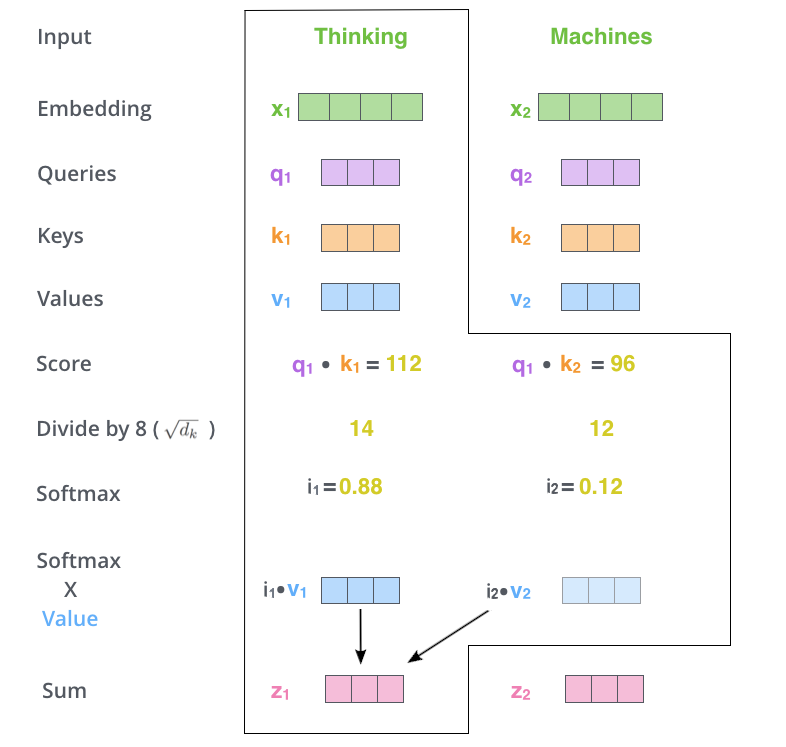
\includegraphics[width=\linewidth]{img/self-attention-output-altered.png}
%   \end{center}
%   \vspace{-0.5cm}
  \caption[Principle of self-attention]{Principle of self-attention. The creation of contextual embedding $z_1$ for the input word \textit{thinking} in the context \textit{thinking machines}. Similar procedure with substitution $q_1 \rightarrow q_2$ in the calculation of Score is done to create the contextual embedding $z_2$ of the word \textit{machines}.  Source \parencite{ilustrtran}, altered. }
  \label{fig:selfatt}
\end{figure}

\vspace{0.5cm}
{\parindent=0pt
    The keys and values may belong to words in a completely different sequence. In that case, it is called simply attention (no longer self-attention). Attention between the hidden state and the sequence generated so far is used in the decoder layers of transformers.
}

\vspace{0.5cm}
{\parindent=0pt
This whole process can be implemented in standard tensor operations that are used in neural networks and works well with backpropagation.
}

\subsubsection{Multi-head attention}
Multi-head attention expands the principle of attention by creating multiple query, key, value triplets. Each one is called a head. This is done to let each head specialize in its own part of the analysis. Each head has its own representation space and can convey different information more easily. This approach improves the overall performance of the model.

\subsubsection{Feed-forward layer}
The output from the self-attention layer gets transformed by a single layer feed-forward network. Its dimension is bigger than the embedding dimension. It is then cast back into the original size. Each self-attention token embedding gets processed independently by the same layer. 

\subsubsection{Residuals}
Both sublayers have a sort of bypass that allows for the flow of information unchanged by the layer. It is summed with the sublayer output and then normalized, so the network can train how much information should bypass it without escalating the output values.

\subsubsection{Stacking}
In order to uncover deep dependencies, the transformer uses multiple encoder layers. Each one can create a higher level of abstraction, similar to convolutional layers in image processing.

\subsection{Decoder layer}
Because decoder layers are not used in the BERT architecture, we will not describe them fully. They recursively generate the output sequence using an attention representation of the sequence generated so far as queries into the hidden representation of the encoders.

\subsection{Usage}
This architecture, in theory, allows for the creation of universal language independent representation of sentences. Each language has its encoder and decoder, and we can connect any two of those to create a machine translation model between these two languages. 


% \section{GPT}
% TODO

\section{BERT}
BERT is a language model developed by Google in 2018~\parencite{bert}. BERT stands for Bidirectional Encoder Representations from Transformers, meaning it uses the encoder part of a transformer\footnote{See Section \ref{sec:transformer}} for creation of bidirectional contextual word embeddings. 

BERT is based on the idea of transfer learning. It has to be pretrained on a lot of data first, and then it can be fine-tuned relatively quickly for a broad range of downstream tasks. Google suggests two self-supervised tasks for the pretraining, which can be automatically generated from a corpus that contains sentence and document separators. Adapting the model for downstream tasks is done by attaching additional layers on the core part of the model.  

At the time of release, the model achieved state-of-the-art results in many NLP tasks \parencite{bert}. 

\subsection{Architecture}
\label{sec:bert_arch}
The BERT architecture consists mainly from the encoder part of the transformer. We will use these letters to annotate its parameters (Figure \ref{fig:bert}). The mentioned sizes correspond to the BERT base model.
\begin{itemize}
\itemsep0em 
\item $V$ -- vocabulary size (30 000)
\item $W$ -- maximum length of the input sequence (512)
\item $L$ -- number of encoder layers (12)
\item $H$ -- hidden size, dimension of the encoder attention vectors (query, key, value), dimension of the output embedding (768)
\item $I$ -- intermediate size, dimension of the feed-forward part of the encoder (3072)
\item $A$ -- number of attention heads (12)
\end{itemize}


\begin{figure}[h]
  \begin{center}
    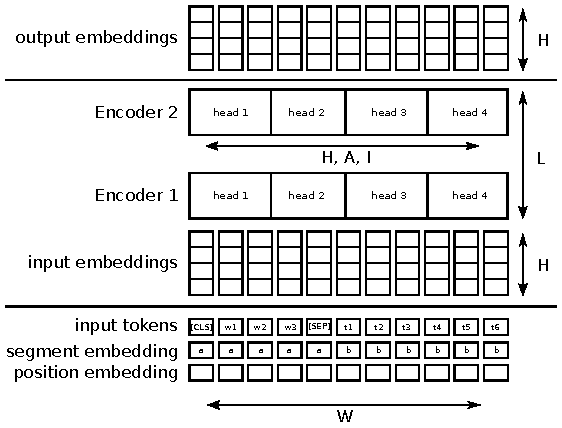
\includegraphics[width=\linewidth]{img/bert_emb.pdf}
  \end{center}
  \vspace{-0.5cm}
  \caption{BERT architecture and parameters}
  \label{fig:bert}
\end{figure}

\subsubsection{Tokenization}
BERT uses a WordPiece tokenizer\parencite[Section 4.1]{google-translation}. WordPiece is a simple tokenizer which uses a greedy algorithm to split each word into tokens. Its vocabulary has two parts: starting tokens (whole words or prefixes) and continuation tokens (suffixes and infixes). For example, the word flying is split into tokens \texttt{fly} and \texttt{\#\#ing}.

Because WordPiece is Google's internal tool, they released only the tokenization process and not the vocabulary creation process, so potential new models had to create their own vocabulary files.

Google later released an improved version called \nobreak{SentencePiece} (more details in Section \ref{sec:sentencepiece}). 


\subsubsection{Model input}
The input tokens are first one-hot encoded and then projected to a vector of dimension $H$. This word embedding is, similarly to the transformer architecture, initialized randomly and learned during pretraining.

The first input token is always \texttt{[CLS]}. Because of the contextuality of the model, its embedding can contain information from the whole input sequence. The embedding of the \texttt{[CLS]} is usually used in classification tasks.

It is often important to know in which part of the sequence a particular token is. To do this, BERT uses position embeddings as a parallel input to the tokens.

Some NLP tasks such as question answering require the model to be able to accept multiple sequences as an input (<Question, Paragraph>). BERT architecture solves this in two ways. The first is to use a special \texttt{[SEP]} token to separate the sequences. The second is segment embedding. The segment embedding is a parallel input to the tokens, and it shows into which sequence the token belongs. This embedding is learned during the training. 

All three embeddings are summed together (input embedding) and are fed to the encoder layers. Each resulting vector is still just a function of one token (and its position and segment); it does not use its context at this point.

The tensor dimension of the compound input embedding is $(W, H)$.

\subsubsection{Encoder layers}
The encoder layers each perform multi-head attention on each token the same way as in the transformer\footnote{See Section \ref{sec:encoder} for a detailed description of the encoder layer.}. This process is what creates the contextual embeddings. There are $L$ encoder layers, each one with $A$ heads which share $H$ neurons together (each head has $\frac{H}{A}$ neurons (the dimension of querry, key and value) -- in the case of BERT$_\text{base}$ it is 64). The feed-forward part of each attention layer has the size $I$. 

As in the transformer, the same weights are applied on all the input embeddings.

The output from the encoder layers is a tensor of dimensions  $(W, H)$.

\subsubsection{}

Unlike ELMo, which has distinct left to right and right to left passes, or GPT\parencite{gpt}, which has only the left context, BERT has a truly bidirectional context. (Figure \ref{fig:contextual_models})

\begin{figure}[h]
  \begin{center}
    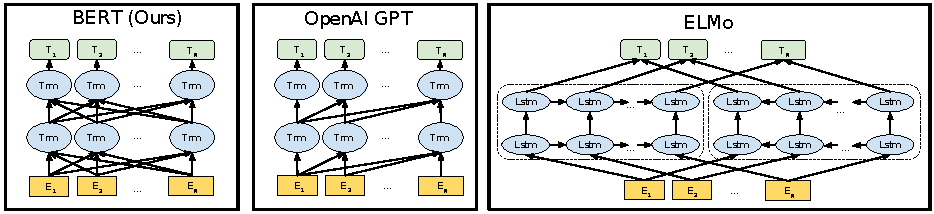
\includegraphics[width=\linewidth]{img/contextual_models.pdf}
  \end{center}
  \vspace{-0.5cm}
  \caption[Architecture differences of contextual models]{\centering Architecture differences of contextual models.\newline{}Source \parencite[page 13]{bert}}
  \label{fig:contextual_models}
\end{figure}



\subsection{Pretraining}
\label{sec:bert_pretraining}
BERT uses two tasks for pretraining.

\subsubsection{Masked language model (MLM)}
Traditional language models are usually trained by predicting the next word in a sequence. To fully utilize and train the bidirectional contextuality of BERT, this training objective is altered. The input is the whole sequence, but with a portion of the tokens hidden or ''masked'' (usually 15 \%). The goal is to predict the original token. For example: \texttt{the cat climbed a~tree~.}~$\xrightarrow{}$~\texttt{the cat climbed a [MASK] .}

This is implemented simply by adding a token classifier on top of the output token embeddings (the core part). It predicts the original masked tokens from the whole dictionary.

Because the \texttt{[MASK]} tokens are only present during pretraining and never for the downstream tasks, the model should get used to not seeing them. The solution proposed in the BERT paper \parencite{bert} is not to always replace the input token with \texttt{[MASK]} token (80 \%), but sometimes use a random token (10 \%) or the correct token (10 \%).  

\subsubsection{Next-sentence prediction (NSP)}
\label{sec:nsp}
To force the model to create long-distance dependencies and to prepare it for multi-input-sequence tasks, the second pretraining objective is next-sentence prediction. Given a pair of sentences, the goal of this task is to decide whether the second sentence was in the original text directly after the first one.  The model uses the contextual embedding of the \texttt{[CLS]} token (which is always the first input token) in a binary classifier to answer this task.

\vspace{1em}
{\parindent=0pt
Both tasks are trained together and at the same time. An example of their input can look like this:
}
\newline
{\footnotesize\texttt{[CLS] the cat climbed a [MASK] . [SEP] than it jumped down .}}
\newline
Or a negative example for NSP:
\newline
{\footnotesize\texttt{[CLS] the cat climbed a [MASK] . [SEP] there are many \newline
tests [MASK] primality .}}


\subsection{Fine-tuning}
Fine-tuning is the process of adapting the pretrained BERT model to a different task then it was pretrained on. 

The first step is modifying the task's input, so it fits the BERT inputs and somewhat resembles the pretraining tasks. This is possible for many tasks, because BERT supports multiple input sequences. Because of its bidirectional nature and fixed width, BERT is not suitable for text generation tasks (whereas GPT\parencite{gpt} is).

The second step is adding additional layer(s) on top of the core (on top of the output embeddings) that are able to answer the task. This usually means adding a classification layer on the output embedding of the first token (\texttt{[CLS]}) if we want to classify the whole input (entailment, sentiment analysis). Or using all the output token embeddings in other ways specific to the token level task (sequence tagging, question answering). An example of modification for question answering is described in Section \ref{sec:qaarch}

The final step is to train the modified model on the task-specific data. All weights are trained during this process.

The fine-tuning process is much faster than the pretraining.  Devlin et al. \parencite{bert} state 16 TPUs for 4 days vs 1 TPU for 1 hour (more than 300x faster)

Examples of possible downstream tasks include all GLUE tasks \parencite{glue}, text classification, sequence tagging, paraphrasing, entailment, question answering, \dots

\subsection{Achievements}
At the time BERT was released (autumn 2018) it achieved these results.

\textbf{GLUE}: Fine-tuned BERT$_\text{base}$ models surpassed all previous models on all the GLUE \parencite{glue} tasks except for the problematic WNLI \parencite[Table 1]{bert}. The performance of BERT$_\text{large}$ was even better.

\textbf{SQuAD} \parencite{squad}: An ensemble model of fine-tuned BERT$_\text{large}$ achieved best results for SQuAD v1 \parencite[Table 2]{bert} and single  fine-tuned BERT$_\text{large}$ model exceeded all previous models (but not human performance) at SQuAD v2\parencite[Table 3]{bert}. 

\section{ALBERT}
In 2019 Lan et al. from Google released a leaner version of BERT called ALBERT~\parencite{albert}, which has much fewer parameters and achieves better performance. Because ALBERT is faster than BERT, it can be trained for a longer time with a bigger model on a bigger corpus. They claim ALBERT is 18 times smaller and achieves similar performance as BERT in 3/5 of the training time.

\subsection{Differences from BERT}
\label{sec:albert_pretraining}
Even though most of the model is the same as BERT (see Section \ref{sec:bert_arch} for the description of BERT), Lan et al. made three main improvements to ALBERT.

\subsubsection{Factorized embedding parameterization}
ALBERT has an additional token embedding layer between the inputs and the encoder layers. In BERT, the input word embedding size is directly tied to the size of the hidden layer $H$. Increasing the size of the hidden layer improves the model performance, but also adds many weights, because the dictionary is large. ALBERT adds an additional parameter $E$ -- size of the input embedding. By uncoupling  the the size of the hidden layer from the embedding size, they allowed increased hidden size $H$ without adding that many weights to the model. The recommended size of $E$ is 128.

\noindent\vbox{\parindent=0pt
 \setlength\abovedisplayskip{0pt}
 \setlength\abovedisplayshortskip{0pt}
 \setlength\belowdisplayskip{0pt}
 \setlength\belowdisplayshortskip{0pt}
For ALBERT$_\text{large}$ with parameters $V = 30000, H=1024, E=128$ the weight count difference is
\begin{equation*}
     30\,000 \cdot 1024 \doteq 30 \text{ M vs. } 4 \text{ M} \doteq 30\,000 \cdot 128 + 128 \cdot 1024
\end{equation*}
}

\vspace{4pt}
{\parindent=0cm
Figure \ref{fig:albert} shows the new architecture.
}

\begin{figure}[hbt]
  \begin{center}
    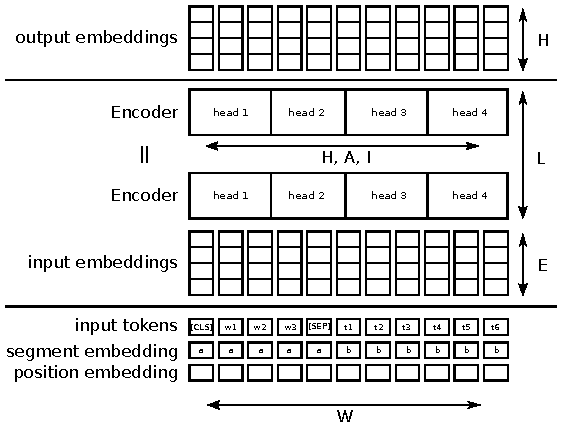
\includegraphics[width=0.9\linewidth]{img/albert.pdf}
  \end{center}
  \vspace{-0.5cm}
  \caption{ALBERT architecture and parameters}
  \label{fig:albert}
\end{figure}

\subsubsection{Cross-layer parameter sharing}
The original BERT uses separate weights for each encoder layer. Previous works have shown (Dehghani et al., 2018 \parencite{uni-trans}) that cross-layer parameter sharing works for standalone transformers, but it was not explored, whether it would work for the pretraining/fine-tuning language model approach. 

The first benefit of parameter sharing is the models have fewer weights (even though they are not faster). This allows for bigger batch sizes during training, which is important \footnote{The importance of batch size is explored in Section \ref{sec:pretr_eval}.}.

When examining how the contextualized embeddings changed in each encoder layer, Lan et al. found out that in BERT the embeddings change a lot and unevenly. Cross-layer parameter sharing causes the embedding change in each layer to be smaller and more consistent. Figure \ref{fig:crosslayer-stability} shows this comparison.  

\begin{figure}[h]
  \begin{center}
    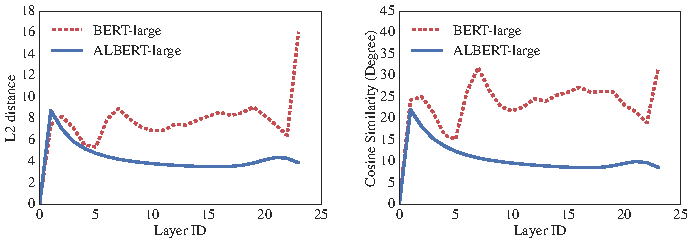
\includegraphics{img/crosslayer-stability.pdf}
  \end{center}
  \vspace{-0.5cm}
  \caption[Effect of cross-layer parameter sharing on embedding stability]
    {Effect of cross-layer parameter sharing on embedding stability. The graphs show L2 distance and cosine similarity of the input and output embedding of each encoder layer for BERT$_\text{large}$ and ALBERT$_\text{large}$. Source \parencite[Figure 1]{albert}}
  \label{fig:crosslayer-stability}
\end{figure}

There are multiple ways to share weights across encoder layers -- only self-attention, only feed-forward or both. The ALBERT architecture shares all the weights.

The impact on performance (Table \ref{tab:crosslayer-performance}) is not that significant, especially for lower $E$, and the benefits outweigh it. Sharing the weights of the feed-forward part has the most significant negative impact.

\begin{table}[h]
  \begin{center}
    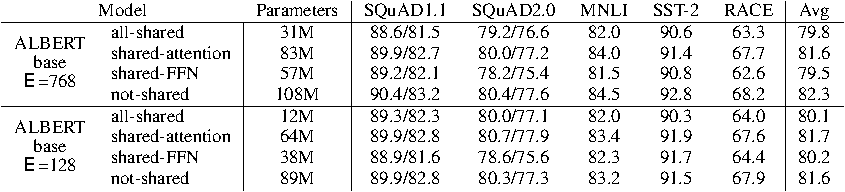
\includegraphics[width=\linewidth]{img/crosslayer-performance.pdf}
  \end{center}
  \vspace{-0.5cm}
  \caption[Effect of cross-layer parameter sharing on performance]{Effect of cross-layer parameter sharing on the performance of English ALBERT. Source \parencite[Table 4]{albert}}
  \label{tab:crosslayer-performance}
\end{table}


\subsubsection{Inter-sentence coherence loss}
The third improvement is changing one of the pretraining tasks. The masked language modeling (MLM) stays unchanged, but the next sentence prediction (NSP, see Section \ref{sec:nsp}) task is replaced by the sentence order prediction (SOP) task.

A negative example of NSP is created by taking the next sentence from a different document than the first one. This sentence has usually a different topic, so it is easier for the model to detect it.

The SOP task is based on inter-sentence coherence, not the topic. Positive examples are created the same way as in the NSP (two consecutive segments from the same document). Negative examples are also created by taking two consecutive segments from the same document, but their order is flipped. This way the topic stays the same in both cases.

Table \ref{tab:sop-vs-nsp} shows the performance impact of this change. We can also see that the model pretrained with NSP is unable to predict the SOP, probably because it observes the easier topic signal. Model pretrained with SOP is able to predict NSP reasonably well (NSP also contains the coherence discrepancy in negative examples)

\begin{table}[h]
  \begin{center}
    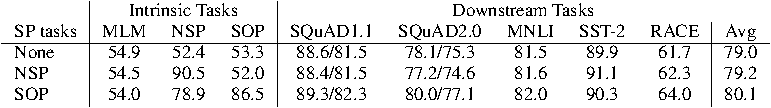
\includegraphics[width=\linewidth]{img/sop-vs-nsp.pdf}
  \end{center}
  \vspace{-0.5cm}
  \caption[Effect of NSP vs. SOP pretraining task]
    {Effect of NSP vs. SOP pretraining task. Source \parencite[Table 5]{albert}}
  \label{tab:sop-vs-nsp}
\end{table}


\subsection{SentencePiece}
\label{sec:sentencepiece}

ALBERT supports a new tokenizer called SentencePiece \parencite{sentencepiece}. SentencePiece is a language-independent tokenizer and detokenizer developed at Google. Unlike BERT's WordPiece tokenizer, SentencePiece has its own C++ and Python version \parencite{spgit}, which can be used to create tokenization models.

The SentencePiece model first needs to be trained. It requires a corpus with sentences. The output is a model file and a vocabulary file, which are self-contained and portable.

The algorithm SentencePiece uses for splitting words into tokens is not greedy. It finds the best possible sentence segmentation with complexity in $O(N \  \text{log}(N))$, where $N$ is the number of characters. SentencePiece supports adding custom tokens (like \texttt{[CLS]}) and standalone tokens.


\subsection{Achievements}

Similarly to BERT, at the time of release (autumn 2019) ALBERT achieved state-of-the-art result on GLUE \parencite{glue} and SQuAD \parencite{squad} (\parencite[Tables 9 and 10]{albert}).

In addition, ALBERT improved the best performance for the RACE dataset \parencite{race}.


% ####################################
% ####################################

\chapter{Czech ALBERT}
This chapter contains the description and details the creation of Czech language models based on the ALBERT architecture. The resulting models are evaluated in Chapter \ref{sec:eval}.

\section{Other language models suitable for Czech}
\label{chap:multimodels}
There are two published transformer-based language models that support the Czech language. 

\subsection{Multilingual BERT}
Multilingual BERT was released by Google along with the original English BERT models \parencite{multibert}. It supports 104 languages and has the same parameters as the BERT base model (except dictionary size). Even though there are not many full Czech words in its vocabulary, the WordPiece tokenizer enables the model to split words into multiple tokens.

\subsection{Slavic BERT}
Slavic BERT is an adapted version of the Multilingual BERT developed by the Moscow Institute of Physics and Technology \parencite{slavicbert}. It is specialized for four languages (Czech, Russian, Bulgarian and Polish). It has bigger vocabulary overlap with the Czech language than the Multilingual BERT.

\vspace{1em}

{\parindent=0cm
For comparison of vocabulary overlap see tables \ref{tab:vocab-nov-compare}, \ref{tab:vocab-prop-compare}, and \ref{tab:vocab-sqad-compare}
}


\section{Source code and repository}
Scripts and libraries I used for this thesis are in a GitHub repository \url{https://github.com/zepzep/csalbert} \parencite{thesis_repo}.

It contains a fork of the ALBERT repository released by Google \parencite{albert_repo}, the scripts for corpus preprocessing, tokenizing, model creation and ALBERT pretraining and fine-tuning.

A minimal working example of fine-tuning of a Czech ALBERT model on a classification task using Keras is included as well.

The pretrained models can be downloaded from \url{https://nlp.fi.muni.cz/projekty/czech_albert/}.


\section{Corpus and text preprocessing}
\subsubsection{Corpus}
For pretraining, I chose the csTenTen17 corpus created by Vít Suchomel at the NLP Centre, Masaryk University, Brno \parencite{tenten1}, \parencite{tenten2}. It contains 10 billion words gathered from a web crawl in 2015--2017.  Even though all sentences are tagged with parts of speech, I only used the raw text. ALBERT pretraining requires text split into documents and sentences. The resulting text file has one sentence on each line, and documents are separated by an empty line. It takes up 72 GB. 

To extract the text from the compressed corpus, I used the script \href{https://github.com/ZepZep/csalbert/blob/master/corpus/sentences_from_raw_vert.py}{\texttt{csalbert/corpus/sentences\_from\_raw\_vert.py}}.

\subsubsection{Text preprocessing}
\label{sec:text_preproc}
The Czech text preprocessor does the following steps:
\begin{itemize}
\itemsep-0.3em 
\item unify numbers: each numeral is replaced by the \texttt{\#} symbol.
\item unify dashes: all dash variants are replaced by the ASCII \texttt{-}
\item unify quotation marks: all variants are replaced by the ASCII \texttt{'}
\item remove all unknown characters: removes all characters but the Czech alphabet and \texttt{'.,!?\%()-'\#: '}
\end{itemize}

{\parindent=0cm
Based on the model settings, the text may be converted to lower case.

\vspace{1em}
For preprocessing, I used the script \href{https://github.com/ZepZep/csalbert/blob/master/corpus/cspreproc.py}{\texttt{csalbert/corpus/cspreproc.py}}.
}

\subsubsection{Example}
\begin{verbatim}
vydejte se z malé skály na vyhlídku nad řekou jizerou.
prozkoumejte tajemný pantheon a zdolejte hrad frýdštejn.
pomozte místní víle a jejímu kamarádovi skřítkovi.
při tom vyřešte ## úkolů a najděte poklad.

a) závodníci kategorií juniorů (#### - ####) mohou v ...
prvním stupněm soutěže je krajská soutěž (včetně ...
druhým stupněm soutěže je semifinále mistrovství čr.
\end{verbatim}

\subsubsection{SentencePiece}
A SentencePiece model is needed for the text tokenization. It can be trained from the same text data that is used in ALBERT pretraining. Because tho whole dataset is unnecessarily big, I used only 10\,000\,000 sentences (1 GB) from the preprocessed dataset.

ALBERT needs some special tokens that do not appear in normal text (like \texttt{[CLS]} and \texttt{[SEP]}). We need to specify this to the SentencePiece trainer, as well as user-defined standalone characters, that are always tokenized separately (like parenthesis or quotation marks).

The dictionary size I chose is 30\,000. This is the same size English ALBERT used. Czech language would probably benefit from bigger dictionary than English, because it is morphologically more diverse, but because of performance reasons, I decided to let it be the same size.

The script I used to train the SentencePiece model is \newline
\href{https://github.com/ZepZep/csalbert/blob/master/corpus/mk_sentencepiece.py}{\texttt{csalbert/corpus/mk\_sentencepiece.py}}.

\section{Pretraining process}
\subsubsection{Creating pretraining data}
Before we can begin pretraining the model, we need to create the data for the pretraining tasks. The ALBERT repository provides a script (\href{https://github.com/ZepZep/csalbert/blob/master/albert/create_pretraining_data.py} {\texttt{csalbert/albert/create\_pretraining\_data.py}}) for this. It creates a TFRecords file, which is then used in pretraining. The script is written in pure Python and does not use many vectorized operations. Because it needs to process gigabytes of text, it is slow and memory intensive. The script does not support parallelism on its own.

In order to process the data more quickly, I split the corpus and ran the script in parallel on each part using GNU Parallel \parencite{parallel}. Despite that, it would take more than 4 days to create pretraining data from the whole csTenTen corpus. I used only 1/4 of the corpus and split it into 34 pieces. Each resulting piece has around 1 GB. The configuration can be found in \href{https://github.com/ZepZep/csalbert/blob/master/pretraining/create_pretrain_data.sh}{\texttt{csalbert/pretraining/create\_pretrain\_data.sh}}.

Figure \ref{fig:pretraining-data} shows one training example. \texttt{input\_ids} are the token ids of the input paragraph. Its length is always the same as the model width $W$. \texttt{tokens} are just translated \texttt{input\_ids} for illustration; they are not saved to the training file.

\texttt{input\_mask} is used in sequences shorter than the model width, it denotes where the padding starts. \texttt{segment\_ids} are used for segment embeddings. \texttt{token\_boundary} shows which tokens are at the word beginning. \texttt{masked\_lm\_ids} and \texttt{masked\_lm\_weights}, are used in the MLM task.\texttt{next\_sentence\_labels} mark whether the two input segments are in the correct order for the SOP task.


\begin{figure}[h]
    \caption{Example of pretraining data}
    \label{fig:pretraining-data}
    \centering
    \makebox[\textwidth][c]{
        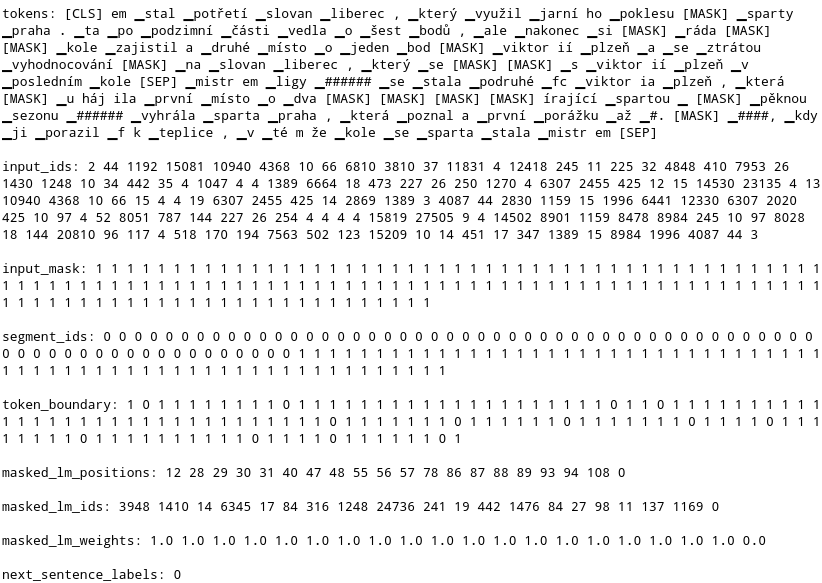
\includegraphics[width=\textwidth]{img/pretraining.png}
    }
\end{figure}



\subsubsection{Model pretraining}

The base pretraining script is located in
\href{https://github.com/ZepZep/csalbert/blob/master/albert/run_pretraining.py} {\texttt{csalbert/albert/run\_\linebreak{}pretraining.py}}. The script is able to both train the model and evaluate it on the pretraining tasks, but not at the same time.

To make it easier, I created a console application (\href{https://github.com/ZepZep/csalbert/blob/master/pretraining/autobert.py}{\texttt{autobert}}) which runs two instances of the script at the same time (one for pretraining, one for evaluation) and presents the output from both in a readable format. It uses yaml config files for model parameter definition and accepts arguments like path to training dataset or number of training steps to train for.

The evaluation results are logged using TensorBoard \parencite{tensorboard} log files. 
To view them, we need to start a local TensorBoard server and connect to it with a web browser. Figure \ref{fig:tb-vis} shows some examples of visualizations that TensorBoard offers. They are updated in real-time during the training, but they can also be viewed later.

\begin{figure}[b!]
    \caption{TensorBoard visualization of pretraining of \textit{csbase4}. }
    \label{fig:tb-vis}
    \centering
    \makebox[\textwidth][c]{
        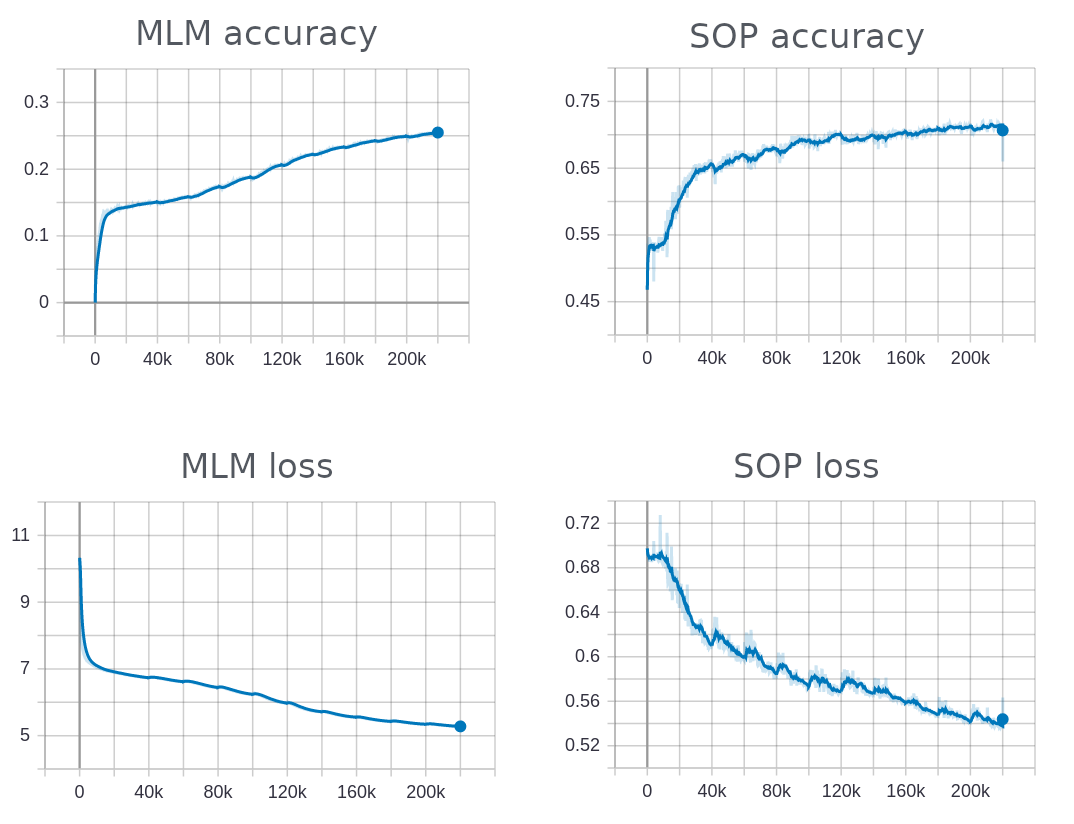
\includegraphics[width=\textwidth]{img/tb_csbase4.png}
    }
\end{figure}

The default English tokenization is not suitable for the Czech language so I had to alter it to comply with the preprocessing described in Section \ref{sec:text_preproc}. 

\subsubsection{MetaCentrum}
Because pretraining needs a lot of computing power, I used MetaCentrum servers. MetaCentrum is a Czech national grid infrastructure which grants academic and research organizations and individuals access to computing and data storage \parencite{metacentrum}. 
MetaCentrum offers machines from many connected clusters with different capabilities.

Pretraining of big neural networks requires powerful GPUs. The \texttt{adan}\footnote{\url{https://wiki.metacentrum.cz/wiki/Cluster_Adan}} cluster offers machines with 2 nVidia Tesla T4 16GB GPUs each. I used this cluster for the pretraining and finetuning.

\vspace{1em}
{\parindent=0cm
ALBERT is written for TensorFlow\footnote{\url{https://www.tensorflow.org/}} 1.15.2. It is not trivial to install an exact version of TensorFlow for GPUs with all of its dependencies without root access. MetaCentrum's module system supports several TensorFlow versions, but it is not perfect and I was not able to get everything working. 
}

The suggested course of action, which I opted for, is to use a virtualized TensorFlow Docker container. I created a container based on \texttt{tensorflow/tensorflow:1.15.2-gpu-py3-jupyter}\footnote{
\href{https://hub.docker.com/layers/tensorflow/tensorflow/1.15.2-gpu-py3-jupyter/images/sha256-2c2ddc9780724ee528757f44beb16dac302a09ee7eb4e333b7dd85404597fdd9}
    {\texttt{https://hub.docker.com/r/tensorflow/tensorflow/tags}}
}, built it and installed all required packages using Docker\footnote{\url{https://www.docker.com/}} and Singularity\footnote{\url{https://sylabs.io/singularity/}}.

MetaCentrum machines also use a hierarchy of storage. Long-term user storage runs on different machines and is slow. The script \href{https://github.com/ZepZep/csalbert/blob/master/pretraining/pretrain.sh}{\texttt{csalbert/pretraining/pretrain.sh}} copies all needed files to a fast local SSD, starts the pretraining in the virtualized container, and after it is finished, the script copies the trained model back to long-term storage. It creates a local TensorBoard server as well. 

I used the GNU Screen\footnote{\url{https://www.gnu.org/software/screen/}} program to allow me to troubleshoot. This way I could connect to the machine that was currently training the model via ssh and inspect the running processes. Forwarding the TensorBoard port also allowed me to view the training progress and current performance.

The last step is to create and queue the jobs so that MetaCentrum can schedule and execute them. Because there is a 24-hour time limit on each job, I needed to split them into smaller pieces. The pretraining dataset is already split because of processing parallelism. I created one job per dataset piece. It takes approximately 3 hours to train 1 epoch over one dataset piece for the smaller models, 6 hours for the large ones (see Table \ref{tab:pretrain-speed} for speed comparison). The jobs were created with dependencies on one another so they would be executed linearly. The implementation is in the script \href{https://github.com/ZepZep/csalbert/blob/master/pretraining/enqueue.sh}{\texttt{csalbert/pretraining/enqueue.sh}}.

 The pretraining took 2\,--\,5 days, depending on the model. 
 

\section{Adapting the model for downstream tasks}
\label{sec:adapting-finetuning}
Fine-tuning the pretrained model is much faster than the pretraining itself. I was able to use my home computer with GTX 1060 6GB as well as MetaCentrum machines. One epoch on the Propaganda dataset takes 3\,--\,8 minutes (single task), and one epoch on the SQAD database takes 4\,--\,9 minutes.

For easier visualization and faster design process of the fine-tuning tasks I used Jupyter notebooks\footnote{\url{https://jupyter.org/}}.

% I include the bare scripts in the repository as well.

\subsubsection{Classification}
Even though ALBERT repository offers a script for text classification (as well as GLUE evaluation), it is written in older TensorFlow and is difficult to adapt.

Luckily there is a python module called \texttt{bert-for-tf2}\footnote{\url{https://github.com/kpe/bert-for-tf2/}} which enables fine-tuning of transformer models like BERT, adapter-BERT and ALBERT in TensorFlow version 2. TensorFlow 2 has better integration with the high-level neural network framework Keras\footnote{\url{https://keras.io/}}, which allows an easier and faster neural network design process. 

The Jupyter notebook \href{https://github.com/ZepZep/csalbert/blob/master/novinky/novinky_finetune.ipynb}{\texttt{csbase/novinky/novinky\_finetune.ipynb}} was used for creation, fine-tuning and evaluation of novinky.cz models. The \href{https://github.com/ZepZep/csalbert/blob/master/propaganda/propaganda_finetune.ipynb}{\texttt{csbase/propaganda/propaganda\_finetune.ipynb}} notebook was used for Propaganda.

\subsubsection{Question answering}
Preprocessing and postprocessing for question answering is much more complicated than for text classification. The ALBERT repository provides the script \href{https://github.com/ZepZep/csalbert/blob/master/albert/run_squad_v2.py}{\texttt{csalbert/albert/run\_squad\_v2.py}}, which deals with many of the problems. It is however designed for the English SQuAD dataset so I had to transform the data from the Czech SQAD dataset and adapt the script.

\vspace{1em}
{\parindent=0pt
The following scripts were used to process the Czech QA: 
\begin{itemize}
    \setlength{\itemsep}{0.1em}
    
\item \href{https://github.com/ZepZep/csalbert/blob/master/sqad/sqad2json.ipynb}
    {\texttt{csalbert/sqad/sqad2json.ipynb}} 
    -- extract the data from the SQAD database and create the Czech QA dataset

\item \href{https://github.com/ZepZep/csalbert/blob/master/sqad/train_sqad.sh}
    {\texttt{csalbert/sqad/train\_sqad.sh}}
    -- fine-tune a Czech ALBERT model on Czech QA dataset

\item \href{https://github.com/ZepZep/csalbert/blob/master/sqad/train_sqad.sh}
    {\texttt{csalbert/sqad/predict\_sqad.sh}}
    -- choose and evaluate the best model and create top predictions
    
\item \href{https://github.com/ZepZep/csalbert/blob/master/sqad/sqad_results.ipynb}
    {\texttt{csalbert/sqad/sqad\_results.ipynb}}
    -- Jupyter notebook for more complex evaluation and visualization

\end{itemize}
}

\subsubsection{Keras integration}
To enable other people to fine-tune and use Czech ALBERT models, there is a minimal working example of a text classifier. It uses the \texttt{bert-for-tf2} Python module and was tested on Python 3.8 and TensorFlow 2.2. The implementation is in the Jupyter notebook \newline
\href{https://github.com/ZepZep/csalbert/blob/master/classification/classification.ipynb}{\texttt{csalbert/classification/classification.ipynb}}.

\subsubsection{Multilingual models}
To be able to compare the Czech ALBERT models to the Multilingual models, I needed to run similar experiments on them as well. The \texttt{bert-for-tf2} module is able to work with both BERT and ALBERT so, for the text classification task, the adaptations were straightforward. However because the BERT models are much bigger, I had to fine-tune them on MetaCentrum.

The adaptation for question answering was more complex. I used the original BERT repository\footnote{\url{https://github.com/google-research/bert}} and the script \href{https://github.com/google-research/bert/blob/master/run_squad.py}{run\_squad.py}. I had to alter the source code in a similar way as the ALBERT source code to fix the English tokenization. The execution scripts for fine-tuning and evaluation are \href{https://github.com/ZepZep/csalbert/blob/master/sqad/bert_train_sqad.sh}
    {\texttt{csalbert/sqad/bert\_predict\_sqad.sh}} and 
\href{https://github.com/ZepZep/csalbert/blob/master/sqad/bert_train_sqad.sh}
    {\texttt{csalbert/\linebreak{}sqad/bert\_predict\_sqad.sh}}

% \clearpage
\section{Models and their parameters}

The training process and model parameters have evolved over the course of this project. For the evaluation, I chose three models from the last iteration -- a base model (\textit{csbase3}), a wide model (\textit{cslarge3}), and a model with more weights (csbase4). All their parameters are shown in Table \ref{tab:pretrain-speed}. Multilingual models and the ALBERT base models are included for comparison.

\begin{table}[h]
\centering
\footnotesize
\makebox[\textwidth][c]{
\begin{tabular}{r|c|c|c|c|c|c|c|c|c}
        Model name
        & \rotatebox[origin=l]{90}{vocab size $V$}
        & \rotatebox[origin=l]{90}{sequence length $W$} 
        & \rotatebox[origin=l]{90}{heads $A$}
        & \rotatebox[origin=l]{90}{hidden size $H$}
        & \rotatebox[origin=l]{90}{model size [MiB]}
        & \rotatebox[origin=l]{90}{weight count}
        & \rotatebox[origin=l]{90}{training speed [ex/s]\hspace{0.5em}}
        & \rotatebox[origin=l]{90}{batch size}
        & \rotatebox[origin=l]{90}{training examples}
        \\ 
    \toprule
    Multilingual BERT      & 119 K  & 512 & 12 & 768 & 681.2 & 110 M & 4  & 256  & 256 M\footnotemark\addtocounter{footnote}{-1} \\
    Slavic BERT            & 119 K  & 512 & 12 & 768 & 684.2 & 110 M & 4  & 256  & 256 M\footnotemark \\
    ALBERT base            & 30 K   & 512 & 12 & 768 & 126.3 & 12 M  & 12 & 4096 & 512 M \\
    csbase3                & 30 K   & 256 & 8  & 256 & 61.23 & 5.2 M & 75 & 32   & 25 M  \\
    cslarge3               & 30 K   & 512 & 8  & 384 & 64.01 & 5.3 M & 30 & 16   & 4 M   \\
    csbase4                & 30 K   & 256 & 12 & 768 & 134.8 & 11 M  & 26 & 32   & 8 M   \\
\end{tabular}
}
\caption[Model parameters, size and speed]
{Model parameters, size, pretraining parameters and speed.}
\label{tab:pretrain-speed}
\end{table}

\footnotetext{training examples of the English BERT, the actual are unknown.} 

Even though the \textit{cslarge3} is twice as wide as \textit{csbase3}, it has almost the same amount of weights (because the encoder layers apply same transformations to all tokens). However, the training speed is much slower, and batch sizes can be only half as big.

The \textit{csbase4} model has more attention heads (12 vs. 8) and a bigger hidden size (768 vs. 256). It needs more calculations per training example, so it is slower. Despite the bigger weight count, \textit{csbase4} can use the same batch size as \textit{csbas3}, because the weights are in the GPU memory only once, and the width of the model is the same.


Full config files for the models are in 
\href{https://github.com/ZepZep/csalbert/blob/master/pretraining/configs} {\texttt{csalbert/pretraining/\linebreak{}configs}}.





% ####################################
% ####################################

\addtocontents{toc}{\vspace{1\baselineskip}}

\chapter{Evaluation}
\label{sec:eval}
\section{Pretraining evaluation}
\label{sec:pretr_eval}
For comparison of the quality of the Czech ALBERT models I used the multilingual models mentioned in section \ref{chap:multimodels}. I also used the base model of English ALBERT released by Google.
Table \ref{tab:pretr-compare} shows the comparison of performance on pretraining tasks 
\footnote{See Sections~\ref{sec:bert_pretraining} and~\ref{sec:albert_pretraining} for details about the pretraining tasks.}.

Masked language modeling is split into two parts. \textit{MLM word} always masks and predicts the whole word, even if it is split into multiple pieces during tokenization. \textit{MLM tok} masks and predicts single tokens. \textit{MLM tok} is easier because the model can use the rest of the word as a context.

Because BERT uses different second pretraining task than ALBERT (next sentence prediction (NSP) vs. sentence order prediction (SOP)) we cannot directly compare the models in these tasks. The NSP task is easier because the two sentences vary in the theme, SOP requires more semantic comprehension. 

The English ALBERT was never pretrained on Czech text; it is here just as a baseline.

\begin{table}[h]
\centering
\begin{tabular}{r|c|c|c|c}
                           & MLM tok & MLM word & NSP  & SOP  \\ 
    \toprule
    Multilingual BERT      & 0.65     & 0.35      & 0.81 & -    \\
    Slavic BERT            & 0.51     & 0.39      & 0.75 & -    \\ 
    English ALBERT         & 0.35     & 0.35      & -    & 0.62 \\ 
    csbase3                & 0.28     & 0.27      & -    & 0.71 \\ 
    cslarge3               & 0.15     & 0.15      & -    & 0.68 \\ 
    csbase4                & 0.26     & 0.25      & -    & 0.71 \\ 
\end{tabular}
\caption[Performance of transformers on Czech pretraining tasks]{Comparison of Performance of transformers on Czech pretraining tasks. The table shows accuracies of pretraining tasks on a part of the Czech TenTen corpus.}
\label{tab:pretr-compare}
\end{table} % tab:pretr-compare

We can see that the Czech ALBERT models perform worse on the MLM task. Possible reasons for this might be:
%I think it is because of the following reasons:

Both BERT models and English ALBERT were pretrained with much more computing power than the Czech ALBERT models. I had to work with smaller models, and despite that, I estimate that using the current setup on MetaCentrum it would take 5 months to pretrain one model on similar amount of data as English ALBERT. Google used a dedicated TPU cloud with 64 to 512 TPUs (depending on the model size), each with 16 GB of RAM. I was able to utilize only single machine and one GPU at a time.

Another contributing factor is smaller batch size. Because of memory constraints and lack of parallelism I could only use maximum batch size of 32. English ALBERT$_{\text{base}}$ used batch size of 4096 (64 TPUs in parallel each with batch size 64). It has been shown in \parencite[page 27, Figure 11]{batch-size} that if we have enough training data (which we do), bigger batch size leads to better performance (even when the number of total training examples the network sees is the same).

To utilize multiple machines/GPUs, a total rewrite of the pretraining process would be needed. The code Google released is meant for a TPU cloud (which is one of their services) and offers a rudimentary support for single GPU or multiple CPUs. Using CPUs is slower and less efficient than using a single GPU. Because this architecture is very new (autumn 2019), at the time I started working on this project, there were no multi-GPU implementations for ALBERT pretraining available.

Because each model uses a different dictionary, the inputs are tokenized differently. When a word does not appear in the dictionary, it has to be split into multiple tokens. This is most apparent in the case of English ALBERT, where all accented Czech characters (like áěš) are split each into separate token. This means that the model input can fit fewer sentences, and the \textit{MLM tok} task shifts from predicting word in a sentence towards predicting letter or syllable in a word. That is probably why the BERT models are much better at \textit{MLM tok} than \textit{MLM word}.  

% copying

The dictionary overlap is explored in tables \ref{tab:vocab-nov-compare}, \ref{tab:vocab-prop-compare}, and \ref{tab:vocab-sqad-compare}.

\clearpage
\section{Downstream tasks}
The main point of language models is their ability to be adapted for a wide range of problems. The concrete tasks the model is fine-tuned for are called downstream tasks. Even if the model performs well on the pretraining tasks, we cannot say that it will perform well on the downstream tasks. To show the quality and adaptability of the model, we need to evaluate it on some downstream tasks.

I chose two domains for the testing -- text classification and question answering.

\section{Text classification}
\subsection{Model architecture}
In text classification tasks, the model predicts into which class the input text belongs. There may be only two classes (yes/no, binary classification), or there may be more classes (multi-class classification).

Binary classification in neural networks is usually done by having a single neuron with a sigmoid activation in the last layer. The network is then trained using the binary cross entropy loss function. The first class corresponds to the output being close to 0, the second class close to 1.

For multi-class classification, we one-hot-encode the class labels and have one neuron for each class in the final layer. The neurons use the softmax activation function. The neuron with the maximum activation value corresponds to the chosen class.

The input for the classification layer is an internal state of the model. There are multiple ways of connecting the classification layer to ALBERT.

\clearpage
{\parindent=0pt
    The BERT paper \parencite{bert} recommends using only the contextual output embedding of the \texttt{[CLS]} token, which is always supplied as the first input token. I chose this method as well. The resulting architecture is shown in Figure \ref{fig:class-basic}. The numbers in brackets are the dimensions of the input/output tensors of the layers. The depicted starting model is \textit{csbase4}.
}

\begin{figure}[h]
    \caption[ALBERT classification model -- basic]{
        ALBERT modification for classification. The last layer is a 8-class classifier for the Location task in Propaganda dataset. The model is based on \textit{csbase4}.
    }
    \label{fig:class-basic}
    \centering
    \makebox[\textwidth][c]{
        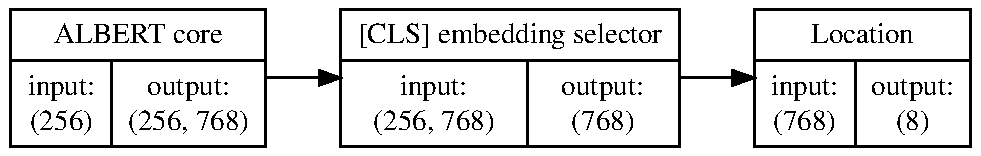
\includegraphics[width=\textwidth]{img/csbase4_base.pdf}
    }
\end{figure}

I also tried to use the output embeddings of all tokens, but the output embeddings consist in total of $H \cdot W$ neurons (for \textit{csbase4} it is 200~K). Connecting a classification layer to them all adds unnecessarily many parameters to the model, which leads to faster overfitting and worse performance. 1D convolutions can reduce the number of parameters, but even with them, the model performed worse. Figure \ref{fig:model-class-use-embed} depicts the internal structure.

\begin{figure}[h]
    \caption[ALBERT classification model -- use all output embeddings]{
        ALBERT classification model that uses all output embeddings. The \texttt{[CLS]} token is used fully; other embeddings are passed through 1D convolution to reduce parameter count. The model is based on \textit{csbase4}.
    }
    \label{fig:model-class-use-embed}
    \centering
    \makebox[\textwidth][c]{
        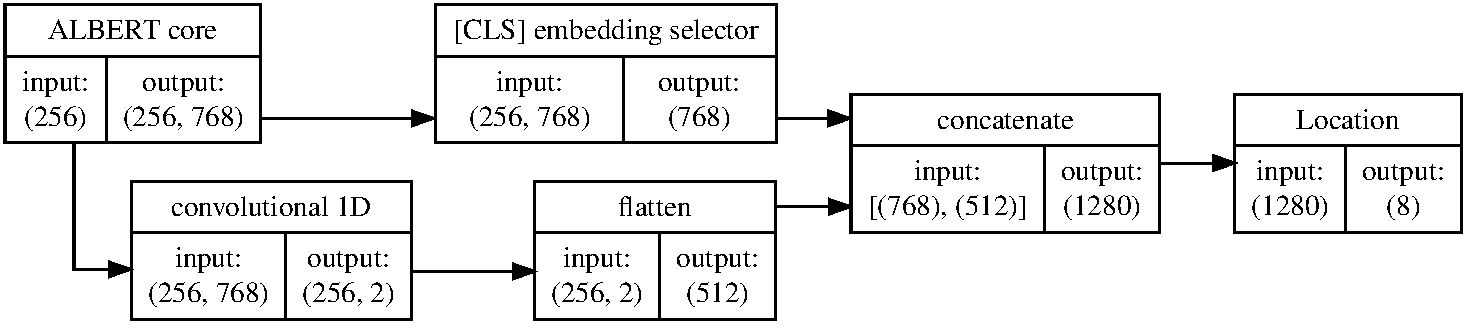
\includegraphics[width=\textwidth]{img/csbase4_conv_alt.pdf}
    }
\end{figure}


When performing multiple classification tasks on the same text, we can branch off the hidden state into multiple classification layers in the same model. This allows the training of multiple tasks at once.
However, it also leads to suboptimal performance because each task starts to overfit at a different time and it is not possible to stop training only one of them. An example of such multi classifier is shown in Figure \ref{fig:model-class-multi}.

\begin{figure}[hbt]
    \caption[ALBERT classification model -- multiple tasks at once]{
        ALBERT classification model that is able to process three tasks at once. The model is based on \textit{csbase4}.
    }
    \label{fig:model-class-multi}
    \centering
    \makebox[\textwidth][c]{
        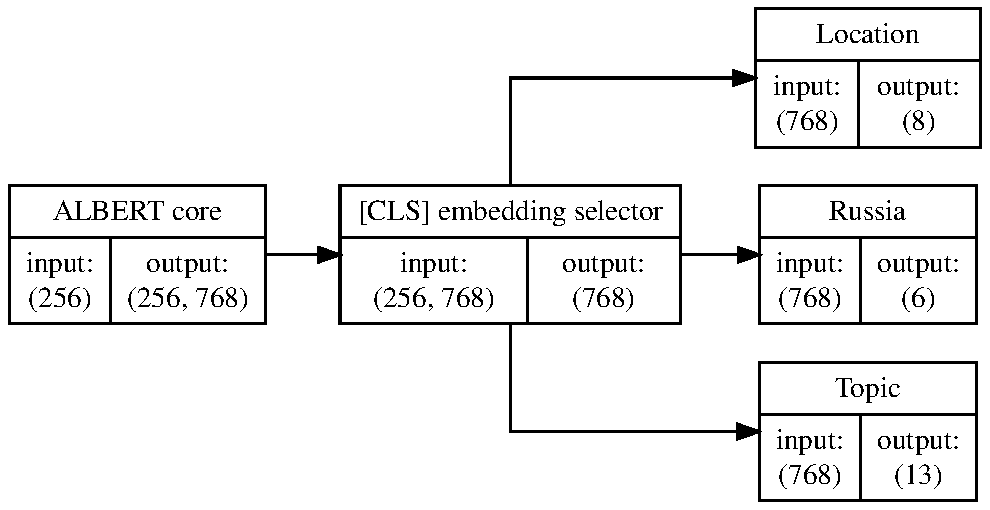
\includegraphics[width=0.8\textwidth]{img/csbase4_split.pdf}
    }

\end{figure}

{\parindent=0cm
For implementation details of text classification see Section \ref{sec:adapting-finetuning}.
}

\subsection{Novinky.cz dataset}

This is a dataset I collected and consolidated from the Czech news server novinky.cz. It consists of 32 000 articles from 8 categories. Each category contains 8 000 articles. The categories are: foreign, crime, culture, economics, cars, internet and PC, traveling, science and education.

% I used this dataset previously for evaluation of a LSTM model which used fasttext embeddings.

The news server was chosen because of its HTML web interface.

Table \ref{tab:vocab-nov-compare} shows the vocabulary coverage of various models on this dataset.

\begin{table}[h]
\centering
\small
\begin{tabular}{r|c|c|c|c|c}
        Novinky.cz
        & \rotatebox[origin=l]{90}{\parbox{2.2cm}{model \\ vocab size}} 
        & \rotatebox[origin=l]{90}{\parbox{2cm}{unique \\ match}}
        & \rotatebox[origin=l]{90}{\parbox{2cm}{unique \\ match [\%]}}
        & \rotatebox[origin=l]{90}{\parbox{2cm}{total \\ match}}
        & \rotatebox[origin=l]{90}{\parbox{2cm}{total \\ match [\%]}}
        \\ 
    \toprule
    Multilingual BERT      & 119 K  & 7 K   & 1.4  & 3.8 M   & 45.8 \\
    Slavic BERT            & 119 K  & 17 K  & 3.6  & 5.9 M   & 71.3 \\
    Czech ALBERT           & 30 K   & 24 K  & 4.9  & 6.3 M   & 79.7 \\ 
\end{tabular}
\caption[Vocabulary coverage on Novinky.cz dataset]
{Comparison of vocabulary coverage on Novinky.cz dataset. The dataset has 490 K unique words and 8.2 M words in total. Only whole word matches are counted, wordpieces are ignored.}
\label{tab:vocab-nov-compare}
\end{table} %tab:vocab-nov-compare

For the classification task, I chose the prediction of article category based on the article description. The article description is the first paragraph of the article, which outlines it's contents.


\newpage
\subsection{Propaganda dataset}
The Propaganda dataset is a collection of 7494 newspaper articles from four selected Czech
digital news servers manually annotated for the presence of specific manipulative techniques \parencite{propaganda}. It was released in 2019  by the NLP Center at Masaryk University.
Each article is supplemented with 18 attributes, such as Blaming or Emotions.

I have chosen 7 tasks with sufficient data for the evaluation whose state-of-the-art models achieve significantly better accuracy than a basic dummy model, which always predicts the most common class. Table \ref{tab:prop-tasks} shows information about these tasks.

\begin{table}[hbt]
\small
\centering
\begin{tabularx}{\linewidth}{r|X|c}
        task & description & classes  \\
    \toprule
        Argumentation   & does the text present facts or arguments to support the main claim? 
            & 2 \\
        Location        &  what is the main location the text talks about?
            & 8  \\
        Source          & is the text presented as being based on a specific source?
            & 2  \\
        Russia          & is the topic related to Russia?
            & 6 \\
        Expert          &  is the text or opinion in the text presented as being supported by an expert?
            & 2  \\
        Topic           &  migrant crisis, domestic politics, etc.
            & 13  \\
        Focus           & foreign, domestic, can’t be determined.
            & 4  \\
        
\end{tabularx}
\caption[Chosen Propaganda tasks]
{List of chosen Propaganda tasks.}
\label{tab:prop-tasks}
\end{table} %tab:prop-tasks

The biggest advantage the Czech ALBERT model has in comparison to the multilingual BERT variants is the vocabulary coverage. Table \ref{tab:vocab-prop-compare} shows the dictionary overlap of the models on the Propaganda dataset.


\begin{table}[t!]
\small
\begin{tabular}{r|c|c|c|c|c}
        Propaganda
        & \rotatebox[origin=l]{90}{\parbox{2.2cm}{model \\ vocab size}} 
        & \rotatebox[origin=l]{90}{\parbox{2cm}{unique \\ match}}
        & \rotatebox[origin=l]{90}{\parbox{2cm}{unique \\ match [\%]}}
        & \rotatebox[origin=l]{90}{\parbox{2cm}{total \\ match}}
        & \rotatebox[origin=l]{90}{\parbox{2cm}{total \\ match [\%]}}
        \\ 
    \toprule
    Multilingual BERT      & 119 K  & 4 K   & 2.5  & 1.6 M   & 47.0 \\
    Slavic BERT            & 119 K  & 16 K  & 9.9  & 2.6 M   & 74.6 \\
    Czech ALBERT           & 30 K   & 21 K  & 13.5 & 2.9 M   & 82.9 \\ 
\end{tabular}
\caption[Vocabulary coverage on Propaganda dataset]
{Comparison of vocabulary coverage on Propaganda dataset. The dataset has 162 K unique words and 3.5 M words in total. Only whole word matches are counted, word pieces are ignored.}
\label{tab:vocab-prop-compare}
\end{table} % tab:vocab-prop-compare



\subsection{Unbalanced classes}
The Novinky.cz dataset was created artificially as an ideal dataset. It contains enough data, and its classes are balanced, meaning there are the same number of examples in each class. This is very important for the training of neural networks, because when the classes are unbalanced, the backpropagation process often leads the network into a worse local optimum \parencite{unbalanced}.

The Propaganda dataset is a real-world dataset. Some tasks have up to ten times as many examples in one class than other class. We cannot easily create new data to balance classes, but there are a few ways to remedy this.

The first way is to ignore the surplus training examples in the majority classes. This is not ideal, because we ignore a big portion of the dataset. The ALBERT model has many parameters and needs a lot of data for successful training. The remaining data would not be enough.

The second way is to clone the examples from minority classes. This is better because we do not waste precious training examples. But if the dataset needs to be static, as is the case for the current implementation of ALBERT, the dataset explodes in size.

\subsubsection{Class weights}
\label{sec:class-weights}
The third way is using class weights\parencite{class-weights}. The basic idea is to \say{put more weight} on less represented classes during training. When backpropagating a training example, the gradient is multiplied by a class weight coefficient. This coefficient is greater than 1 for minor classes and smaller for major classes. This way the, network is influenced more by the minor classes in each step, but because there are more examples from major classes, the influence is balanced in the scope of one epoch.

I chose to use this method because of its simplicity (Keras supports it off the shelf) and its adaptability.

The equation \ref{eq:class-weights} shows the formula I used for calculating the class weights. It ensures that the class-weight-modified learning rate stays the same.

\begin{equation}
\text{class weight} = \frac{\text{dataset size}}{\text{class size} \cdot \text{number of classes}} 
\label{eq:class-weights}
\end{equation}


\subsubsection{Class weights decay}
\label{sec:dynamic-class-weights}
I discovered that modifying the class weights during training can lead to better results. For example, when one class has a much greater class weight because it is badly represented, the model can fixate on this class and is unable to choose a different class.

To fix this, I decided to \say{normalize} the classes a bit (meaning bring them all closer to 1) every epoch. For this, I needed a function which when applied on itself, has limit 1. Example of such a function is the square root function ($\forall x>0: \lim_{n\to\infty} \text{sqrt}^n(x) = 1$). All power functions ($f(x) = x^k; k \in \mathbb{R}$) which satisfy $0 < k < 1$ have this property as well.
I experimented with the value of the exponent and discovered that normalization function $f(x) = x^{0.7}$ works the best.

Table \ref{tab:class-weights-compare} shows the improvements gained by class weights.


\subsection{Evaluation method}
\label{sec:class-eval-method}
The datasets are evaluated with two metrics -- accuracy and weighted f1 score (weighted mean of f1 scores of each label).

The models that were evaluated are the Czech ALBERT models (\textit{csbase3}, \textit{cslarge3} and \textit{csbase4}), the multilingual models (\textit{Multilingual BERT} and \textit{Slavic BERT}) and a \textit{dummy} model. 

The \textit{dummy} model is the simplest model possible, which always predicts the prevalent class. It provides a baseline for the results.

A \textit{noinit} variant of some models is included to test how pretraining effects the results. \textit{noinit} models have the same parameters as their counterparts, but their weights are initialized randomly, nullifying the pretraining. They are trained only on the fine-tuning task.

All models were fine-tuned for 6 epochs, which was enough to overtrain them. 80/20 train/test split was used. The best-performing model on the test set over the entire fine-tuning was chosen as the final model. This procedure has the same effect as early stopping. The reported results are the metrics on the test set for the final model. 

\subsection{Results}
\subsubsection{Novinky.cz}

Table \ref{tab:novinky-results} shows the comparison of evaluated models.

\begin{table}[t]
\small
\begin{adjustbox}{center}
\begin{tabular}{r|c|c|c|c|c|c|c|c|c|c|c}
        novinky.cz
        & \rotatebox[origin=l]{90}{dummy} 
        & \rotatebox[origin=l]{90}{fasttext} 
        & \rotatebox[origin=l]{90}{csbase3 noinit}
        & \rotatebox[origin=l]{90}{csbase3}
        & \rotatebox[origin=l]{90}{cslarge3}
        & \rotatebox[origin=l]{90}{csbase4 noinit}
        & \rotatebox[origin=l]{90}{csbase4}
        & \rotatebox[origin=l]{90}{Mul. BERT noinit}
        & \rotatebox[origin=l]{90}{Mul. BERT}
        & \rotatebox[origin=l]{90}{Slavic BERT noinit\hspace{0.4em}}
        & \rotatebox[origin=l]{90}{Slavic BERT}
        \\ 
    \toprule    % d     
    accuracy    & 12,5 & 78,7 & 85,5 & 90,0 & 90,1 & 83,2 & \textbf{90,9} & 88,0 & 87,3 & 88,2 & \textbf{93,8} \\
    wf1         & 2,8  & 78,7 & 85,4 & 90,0 & 90,1 & 83,2 & \textbf{90,9} & 88,0 & 87,3 & 88,2 & \textbf{93,8} \\
\end{tabular}
\end{adjustbox}
\caption[Evaluation results on novinky.cz dataset]
{Evaluation results on novinky.cz dataset. The table presents accuracy (acc) and weighted f1 score (wf1) of each task in \%. The best values for Czech ALBERT models and for all models are bold. The \textit{dummy} model is a simple classifier that always guesses the most common class.}
\label{tab:novinky-results}
\end{table} % tab:vocab-prop-compare

Because the dataset is well-balanced, the weighted f1 score of real models is very similar to the accuracy.

The \textit{fasttext} \parencite{fasttext} model is presented for comparison as a shallow model. It is much faster but performs worse and the size of the resulting classifier is comparable to the size of the Czech ALBERT models.

We can see that from the Czech ALBERT models, \textit{csbase4} was the most successful. That is understandable because \textit{csbase4} is the biggest of them. However fine-tuning of \textit{csbase4} took almost three times as long as for the \textit{csbase3} whose accuracy is not too far behind.

Because the article descriptions almost always fit into the 256 tokens, \textit{cslarge3} had no significant advantage over \textit{csbase3}.

We can also see that the \textit{noinit} Czech ALBERT models and Slavic BERT perform significantly worse than the pretrained variants. 
From the fact that \textit{noinit Slavic BERT} is worse than the pretrained \textit{csbase3} and the gap between \textit{noinit} accuracy and pretrained accuracy is similar in both models we could infer that with better pretraining the Czech ALBERT models would be more accurate.

Both \textit{Multilingual BERT} models perform worse than the pretrained Czech ALBERT models. This is probably because of the lower vocabulary coverage (see Table \ref{tab:vocab-nov-compare}). The \textit{Slavic BERT}, which has better coverage but the same parameters, performs a lot better. This shows that with inadequate vocabulary and tokenization, not even the strength of this big model can save it. 

A weird phenomenon arises with the \textit{Multilingual BERT} where the \textit{noinit} variant achieves better accuracy than the pretrained one. One explanation might be that the novinky.cz task is highly dependent on specialized use of vocabulary and the general knowledge from pretraining is not useful. The pretrained weights might define different solution space, and it might not be possible to transition to a solution space similar to the \textit{noinit} model solution space using backpropagation. The experiment was repeated multiple times, and these results are consistent. 


\subsubsection{Propaganda}

The propaganda dataset contains diverse tasks that focus on different aspects of text classification. There is no single best model. Table \ref{tab:prop-results} shows the evaluation results.

\begin{table}[hbt]
\scriptsize
\centering
\begin{adjustbox}{center}
\begin{tabular}{r|c|c|c|c|c|c|c|c|c|c|c|c|c|c}
        task & \multicolumn{2}{c|}{\rotatebox[origin=l]{90}{Argumentation \hspace{0.5em}}} & \multicolumn{2}{c|}{\rotatebox[origin=l]{90}{Location}} & \multicolumn{2}{c|}{\rotatebox[origin=l]{90}{Source}} & \multicolumn{2}{c|}{\rotatebox[origin=l]{90}{Russia}} & \multicolumn{2}{c|}{\rotatebox[origin=l]{90}{Expert}} & \multicolumn{2}{c|}{\rotatebox[origin=l]{90}{Topic}} & \multicolumn{2}{c}{\rotatebox[origin=l]{90}{Focus}} \\
 
        classes & \multicolumn{2}{c|}{2} & \multicolumn{2}{c|}{8} & \multicolumn{2}{c|}{2} & \multicolumn{2}{c|}{6} & \multicolumn{2}{c|}{2} & \multicolumn{2}{c|}{13} & \multicolumn{2}{c}{4} \\
   
        metric & acc & wf1 & acc & wf1 & acc & wf1 & acc & wf1 & acc & wf1 & acc & wf1 & acc & wf1 \\
   
   \toprule
        dummy & 57,9 & 42,5 & 35,9 & 18,9 & 60,0 & 45,0 & 66,2 & 52,8 & 57,4 & 41,8 & 28,6 & 12,7 & 58,0 & 42,6 \\
        
        noinit csbase3 & 69,6 & 69,2 & 66,6 & 63,1 & 64,5 & 64,4 & 75,6 & 71,1 & 71,4 & 71,5 & 54,4 & 49,3 & 85,4 & 83,4 \\
        
        csbase3 & 70,2 & \textbf{70,0} & 74,4 & 75,4 & 68,1 & 68,3 & 80,6 & 78,1 & \textbf{73,9} & \textbf{73,2} & 67,8 & 66,5 & 87,0 & 86,4 \\
        
        noinit cslarge3 & 69,6 & 69,5 & 68,5 & 67,3 & 71,9 & 70,8 & 81,8 & 78,4 & 70,6 & 70,4 & 65,9 & 62,8 & 87,4 & 86,2 \\
        
        cslarge3 & 69,6 & 69,7 & \textbf{76,1} & \textbf{75,7} & 71,3 & \textbf{70,8} & \textbf{82,9} & \textbf{80,4} & 72,8 & 72,5 & \textbf{69,7} & \textbf{69,0} & \textbf{88,8} & \textbf{88,1} \\
        
        noinit csbase4 & 68,5 & 67,7 & 72,4 & 71,6 & 67,3 & 67,6 & 80,6 & 77,2 & 71,5 & 71,1 & 63,4 & 62,2 & 85,4 & 84,9 \\
        
        csbase4 & \textbf{72,0} & 68,7 & 76,0 & 74,2 & \textbf{72,0} & 70,3 & 82,0 & 77,7 & 73,5 & \textbf{73,2} & 69,0 & 66,4 & 87,0 & 85,9 \\
        
        noinit Mul. BERT & 68,4 & 68,5 & 74,8 & 74,1 & 70,9 & 70,1 & 81,7 & 79,3 & 72,6 & 72,6 & 65,8 & 63,9 & 88,0 & 87,0  \\
        
        Mul. BERT & 72,4 & 71,1 & \textbf{83,1} & \textbf{82,5} & 73,7 & 72,8 & 82,1 & 80,3 & 77,3 & \textbf{76,7} & 72,4 & 71,3 & \textbf{89,8} & \textbf{89,9} \\
    
        Slavic BERT & 72,6 & \textbf{72,5} & 81,0 & 80,4 & \textbf{75,7} & \textbf{75,7} & 82,1 & 80,0 & 72,6 & 71,8 & \textbf{72,9} & \textbf{72,3} & 89,1 & 89,0 \\

        SOA & \textbf{75,0} & 65,0 & 76,0 & 68,0 & 70,0 & 63,0 & 82,0 & 71,0 & \textbf{81,0} & 73,0 & 71,0 & 64,0 & 87,0 & 77,0 \\


\end{tabular}
\end{adjustbox}
\caption[Evaluation results on Propaganda]
{Evaluation results on the Propaganda dataset. The table presents accuracy (acc) and weighted f1 score (wf1) of each task in \%. The best values for Czech ALBERT models and for all models are bold. The \textit{dummy} model is a simple classifier that always guesses the most common class.}
\label{tab:prop-results}
\end{table} %tab:prop-results

The multilingual models usually achieve the best performance, even better than the SOA\footnote{The \textit{SOA} is the state-of-the-art performance from the Propaganda paper \parencite{propaganda}.}. The Czech ALBERT models are comparable to the SOA, but their weighted f1 score is better, probably thanks to the class weights (see Section \ref{sec:class-weights}).

The \textit{noinit} models perform worse. Once again, most of the pretrained Czech ALBERT models are better than the \textit{noinit Mul. BERT} model. There is also a big gap between \textit{noinit Mul. BERT} and \textit{Mul. BERT}.

On most of the tasks, the performance of \textit{noinit cslarge3} and \textit{noinit BERT} are very similar, which suggests that with better pretraining the \textit{cslarge3} model would achieve higher accuracy. It also probably seems that model width is most important for these tasks because the narrower Czech ALBERT models performed worse. This makes sense because the key phrases/sentences that determine the article's class are sometimes further in the text, and the wider models have better chance to contain them in the input.

\vspace{1em}
{\parindent=0cm
The effect of class weights on fine-tuning with unbalanced dataset is shown in Table \ref{tab:class-weights-compare}. 
}

Three experiments were conducted, one without class weights, one with static class weights and one with dynamic class weights   
The dynamic class weights were normalized in each epoch as described in \ref{sec:dynamic-class-weights}.

We can see that \textit{static class weights} decrease accuracy but improve the f1 score and weighted accuracy. The \textit{dynamic class weights}  keep the increased f1 and weighted accuracy of the \textit{static class weights} and improve the accuracy as well.


\begin{table}[h]
\centering
\begin{adjustbox}{center}
\begin{tabular}{r|c|c|c|c|c|c|c|c|c}
    task & \multicolumn{3}{c|}{Russia} 
     & \multicolumn{3}{c|}{Expert}
     & \multicolumn{3}{c}{Topic} \\
    
    classes & \multicolumn{3}{c|}{6} & 
    \multicolumn{3}{c|}{2} & 
    \multicolumn{3}{c}{13} \\
    
    metric & acc & wf1 & wa & acc & wf1 & wa & acc & wf1 & wa \\
    \toprule
        no weights & 80,2 & 77,2 & 27,8 & 72,3 & 71,7 & 70,5 & 67,1 & 65,5 & 49,2 \\
        
        static weights & 79,7 & \textbf{78,7} & 31,7 & 72,8 & 72,5 & 71,7 & 67,0 & \textbf{66,8} & \textbf{54,4} \\
        
        dynamic weights & \textbf{80,6} & 78,1 & \textbf{32,5} & \textbf{73,9} & \textbf{73,2} & \textbf{71,8} & \textbf{67,8} & 66,5 & 53,6 \\
\end{tabular}
\end{adjustbox}
\caption[The effect of class weights on training]
{The effect of class weights on training. Each task is evaluated on accuracy (acc) and weighted f1 score (wf1) and weighted (balanced) accuracy (wa). All values are in \%. The \textit{csbase3} model was used as a starting point for the fine-tuning.}
\label{tab:class-weights-compare}
\end{table} %tab:class-weights-compare


\clearpage

\section{Question answering}
Question answering (QA) is a reading comprehension NLP task, where the goal is to find an answer to a question in some related context. One of the most famous QA datasets is the English SQuAD (Stanford Question Answering Dataset, \parencite{squad}). SQuAD consists of 500+ Wikipedia articles and more than 150\,000 questions. At the time English ALBERT was released, it achieved the best performance on SQuAD \parencite[Table 10]{albert}, \parencite{squad}. Currently (since April 6th, 2020), the best model also in part uses the ALBERT architecture \parencite{squad}.


\subsection{Czech SQAD dataset}
The biggest Czech QA dataset is called SQAD (Simple Question Answering Database) and was released by Radoslav Sabol et al. at the NLP Center of Masaryk University \parencite{sqad}. Its newest version (v3) contains more than 13 000 questions.

However, SQAD is quite different from its English counterpart. The main difference is that Czech SQAD primarily focuses on the answer selection task (the whole sentence is selected) and not answer extraction task (only the relevant word/phrase is selected). Because of this, the questions are not tied to a specific paragraph as in SQuAD but to whole article, which is much longer. Also, the question density differs significantly. SQuAD usually has at least 5 questions per paragraph and most of SQAD has only 1 question per article.

The architecture of ALBERT is more suitable for the answer extraction task because the whole article cannot fit into the model at once.

Czech SQAD contains the answer extraction data, but it is not perfect. 16 \% of SQAD v3 are yes/no questions, which cannot be answered by simple extraction (if we do not want to select the whole sentence). The answer extractions also sometimes do not appear exactly the same in the text or appear multiple times. Other answers inconsistently contain prepositions (e.g., Since when was cinnamon known in Czech lands? -- [since] 15. century). Capitalization between answer extraction and context is also inconsistent.

Table \ref{tab:vocab-sqad-compare} shows the vocabulary coverage of *BERT models on the SQAD dataset. 

\begin{table}[h]
\centering
\begin{tabular}{r|c|c|c|c|c}
        Czech SQAD
        & \rotatebox[origin=l]{90}{model vocab size \hspace{0.5em}}
        & \rotatebox[origin=l]{90}{unique match}
        & \rotatebox[origin=l]{90}{unique match [\%]}
        & \rotatebox[origin=l]{90}{total match}
        & \rotatebox[origin=l]{90}{total match [\%]}
        \\ 
    \toprule
    Multilingual BERT      & 119 K  & 10 K  & 1.48  & 9.99 M   & 43.7 \\
    Slavic BERT            & 119 K  & 19 K  & 2.80  & 15.2 M   & 66.7 \\
    Czech ALBERT           & 30 K   & 24 K  & 3.61  & 16.7 M   & 73.0 \\ 
\end{tabular}
\caption[Vocabulary coverage on Czech SQAD dataset]
{Comparison of vocabulary coverage on the Czech SQAD dataset. The dataset has 677 K unique words and 22.8 M words in total. Only whole word matches are counted, wordpieces are ignored.}
\label{tab:vocab-sqad-compare}
\end{table} %tab:vocab-sqad-compare


\subsection{Model architecture}
\label{sec:qaarch}

This section describes only high-level concepts, for implementation details see Section \ref{sec:adapting-finetuning}.

\subsubsection{Model input}
The \textit{question} and \textit{context} are tokenized using SentencePiece\footnote{See Section~\ref{sec:sentencepiece}.} and compound into a single sequence in the following way:
\newline \texttt{[CLS] q$_1$ q$_2$ ... [SEP] c$_1$ c$_2$ ... [SEP]} \newline
q$_i$ are the \textit{question} tokens, c$_i$ are the \textit{context} tokens.

In addition, the two segments are marked differently in the segment embedding.

\subsubsection{Model output}
The model adaptation for QA introduces only two new vectors \linebreak $s, f \in \mathbb{R}^H$ of dimension $H$ (hidden size). They are used to calculate the probability of some token being the answer-starting and answer-ending token, respectively. The probability is calculated as a dot product of the output token embedding $t_i$ and the start or end vector followed by softmax over the whole context.

\vspace{-2em}
{\Large$$
\text{P}_\text{start}^i = \frac{e^{s \cdot t_i}}{\sum_j e^{s \cdot t_j}} 
\hspace{3em}
\text{P}_\text{end}^i = \frac{e^{f \cdot t_i}}{\sum_j e^{f \cdot t_j}}
$$}
\vspace{-1em}

The score for a candidate answer span $(i, j)$ is calculated as \linebreak $t_i \cdot s + t_j \cdot f$. The span which satisfies $i < j$ and has the maximal score is selected as the model answer.

The training objective is the sum of the log-likelihoods of the correct start and end positions \parencite[section 4.2]{bert}.

\subsection{Evaluation method}

\begin{samepage}
I chose to evaluate three tasks:
\begin{itemize}
    \itemsep-0.3em 
    \item \textbf{Answer selection} -- Select the sentence which contains the answer from the whole context. 
    \item \textbf{Answer pinpoint} -- Select the exact answer (word, phrase, name, date,~\dots) from the whole context.
    \item \textbf{Answer extraction} -- Select the exact answer (word, phrase, name, date,~\dots) from the answer sentence.
\end{itemize}
\end{samepage}

Answer selection and answer extraction are the same tasks as in the SQAD papers \parencite{sqad}, \parencite{sqadv1}. Answer pinpoint is a task that does both things at the same time.

Each task is evaluated on two metrics: match@k and coverage@k. \textit{k} is the number of candidate answers with the best score that were selected by the model.

\textit{match@1} is the fraction of answers that were selected correctly as the first most probable answer.

Coverage on a single example is calculated as the length of the longest common sequence of characters between answer and prediction divided by the maximum of answer and prediction lengths. \textit{coverage@5} is the mean of coverages by the best prediction in the first 5 predictions.


The models were trained for 20 epochs and similarly as in text classification, the best model on the test set was chosen. The train/test split used was 0.9/0.1. 


\subsection{Results}

Table \ref{tab:sqad-results} shows the evaluation results on the Czech SQAD. 


\begin{table}[h]
\centering
\small
\begin{adjustbox}{center}
\begin{tabular}{rr|c|c|c|c|c|c|c|c|c}
    
        & task & \multicolumn{3}{c|}{answer selection} & \multicolumn{3}{c|}{answer pinpoint} & \multicolumn{3}{c}{answer extraction} \\
        
        %& & \multicolumn{3}{c|}{\Gape[1em]{\parbox{7.5em}{\centering answer sentence \newline selection}}} & \multicolumn{3}{c|}{answer selection} & \multicolumn{3}{c}{answer extraction} \\

        & @ & 1 & 5 & 10 & 1 & 5 & 10 & 1 & 5 & 10 \\
    \toprule
        \cellcolor{thesis@color@tableOdd} & match &
            0,12 & 0,23 & 0,29 & 0,09 & 0,19 & 0,22 & 0,18 & 0,37 & 0,43 \\
        \multirow{-2}{*}{\cellcolor{thesis@color@tableOdd}csbase3}    & coverage &
            0,45 & 0,60 & 0,68 & 0,21 & 0,41 & 0,46 & 0,34 & 0,64 & 0,71 \\
        
        \cellcolor{thesis@color@tableEven} & match &
            0,14 & 0,25 & 0,32 & 0,09 & 0,20 & 0,23 & 0,18 & 0,36 & 0,42 \\
        \multirow{-2}{*}{\cellcolor{thesis@color@tableEven}cslarge3}    & coverage & 
            0,45 & 0,64 & 0,73 & 0,22 & 0,42 & 0,47 & 0,35 & 0,62 & 0,69 \\
        
        \cellcolor{thesis@color@tableOdd} & match & 
            0,17 & 0,29 & 0,34 & 0,10 & 0,23 & 0,25 & 0,23 & 0,42 & 0,51 \\
        \cellcolor{thesis@color@tableOdd}\multirow{-2}{*}{csbase4} & coverage &
            0,47 & 0,69 & 0,76 & 0,25 & 0,45 & 0,50 & 0,43 & 0,66 & 0,75 \\
        
        \cellcolor{thesis@color@tableEven} & match &
            \textbf{0,84} & 0,87 & 0,88 & \textbf{0,64} & \textbf{0,78} & \textbf{0,81} & \textbf{0,75} & \textbf{0,87} & \textbf{0,89}  \\
        \multirow{-2}{*}{\cellcolor{thesis@color@tableEven}multilingual BERT}  & coverage &
            \textbf{0,86} & 0,93 & 0,95 & \textbf{0,83} & \textbf{0,93} & \textbf{0,95} & \textbf{0,89} & \textbf{0,95} & \textbf{0,96}  \\
        
        \cellcolor{thesis@color@tableOdd} & match &
            0,79 & \textbf{0,94} & \textbf{0,96} & - & - & - & 0,38 & - & - \\
        \cellcolor{thesis@color@tableOdd}\multirow{-2}{*}{SOA} & coverage &
            0,79 & \textbf{0,94} & \textbf{0,96} & - & - & - & 0,42 & - & - \\
        
\end{tabular}
\end{adjustbox}
\caption[Evaluation results on SQAD v3]
{Evaluation results on SQAD v3}
\label{tab:sqad-results}
\end{table} %tab:sqad-results

\vspace{1em}

{\parindent=0pt
    The state-of-the-art (SOA) results are from two different papers.
}

Answer sentence selection is from Sabol, Medveď and Horák 2019 \parencite[Table 3]{sqad}. They share only the number for the match metric, but because their model can only select whole sentences, the coverage figures are the same. This paper does not share the results for answer extraction.

Answer extraction figures are from Medveď and Horák 2018 \parencite[Table 1 a)]{sqadv1}. This paper is older and summarizes results from SQAD~v1.1. They share only the exact match and partial match metrics. I used the exact match as match@1 and exact $\text{match} + 0.5 \cdot \text{partial match}$  as coverage@1 (assuming that partial match has, on average, 50\% coverage, the original partial coverage is 0.08).  


The Multilingual BERT outperforms all models if we take only the first answer. It is much better in answer extraction than the SOA model\footnote{However, the SOA models for the answer extraction task were trained only on SQAD v1.1}.

The Czech ALBERT models were unable to achieve the SOA performance. The \textit{csbase4} model is the best of them and slightly improves the SOA answer extraction coverage. Because \textit{csbase4} is the biggest of Czech ALBERT models, it seems that question answering is a harder problem than text classification, and the Czech ALBERT models are too small to be good at it. 

The BERT/ALBERT architecture is probably most suitable for the answer extraction task because single sentences can comfortably fit in the input, and the model is better at selecting smaller answer spans. 

% ####################################
% ####################################

\section{Summary}

Because of insufficient processing power and framework restrictions, I had to compromise with model sizes and the length of pretraining. Despite that, even the small Czech ALBERT models show a lot of potential, and on the classification tasks often achieved state-of-the-art accuracy.

However, they are still overshadowed by the multilingual BERT models, which almost always had the best performance. On the other hand, the Czech ALBERT models are around 10$\times$ faster to fine-tune, and require only a GPU with 6 GB of memory which is much cheaper than the 16 GB GPUs that are required for the BERT models.

Even though fine-tuning on CPUs is a possibility, it is 10$\times$ slower than on the small GPU (AMD Ryzen 7 3700X 8/16 cores/threads, 3.6~GHz vs. GTX 1060 6GB). However, CPUs do not have the problem with insufficient memory because RAM is much cheaper and more expandable than GPU memory.

Question answering is a much harder task than text classification, and the simple Czech ALBERT models are not good at it. The Multilingual BERT excels mainly in the answer extraction task and suggests that bigger models with good pretraining would do better as well.

\section{Possible improvements}
 Because ALBERT is a new architecture, many tools for it are still in development.

The current pretraining method released by Google is unable to utilize multiple GPUs at once. By updating the whole process to TensorFlow 2 it would be possible to make the process more efficient and use as many GPUs as the hardware allows.

TensorFlow 2 has improved pipeline capabilities as well, which would eliminate the need for creating pretraining data beforehand, and the whole pretraining process would be much more flexible.

The third major improvement TensorFlow 2 brings is mixed precision\footnote{\url{https://www.tensorflow.org/guide/keras/mixed_precision}}. It is possible to use only 16 bit floats instead of the usual 32 bit, which effectively doubles the processing speed and available memory. This would allow for bigger batch sizes and longer pretraining. 


% ####################################
% ####################################

\chapter*{Conclusion}
\addcontentsline{toc}{chapter}{Conclusion}

This thesis explored the process of pretraining and evaluation of a new language model called ALBERT for the Czech language. The first chapter focuses on the most common approaches for applying deep artificial neural networks to NLP tasks. The second chapter describes more sophisticated language models used in NLP, including ALBERT and models that lead to it. The third chapter describes the process of training Czech ALBERT models. The fourth chapter contains the evaluation of Czech ALBERT models and comparison with current state-of-the-art models as well as a description of the evaluation tasks.

The Czech ALBERT models were able to achieve state-of-the-art performance for text classification tasks. They were however not good enough for question answering, probably because of their small size and insufficient pretraining.

The pretrained Czech models are 8\,--\,12$\times$ faster (although worse-performing) alternative to the large multilingual models like Multilingual or Slavic BERT. They can be easily fine-tuned for a variety of down-stream NLP tasks. The pretrained models can be downloaded from \url{https://nlp.fi.muni.cz/projekty/czech_albert/}, and the repository \url{https://github.com/zepzep/csalbert} contains examples of their use.

With more processing power and better implementation (TensorFlow 2), the current Czech ALBERT models could be improved, and larger models would be feasible.


% \makeatletter\thesis@blocks@clear\makeatother
%   \phantomsection %% Print the index and insert it into the
%   \addcontentsline{toc}{chapter}{\indexname} %% table of contents.
% %   \printindex

% \appendix %% Start the appendices.
% \chapter{An appendix}
% Here you can insert the appendices of your thesis.

\end{document}
